\begin{center}\large\textbf{Readings: 11.1-11.6 and 11.9-11.11 pg 463 - 515 and 529 - 539}\\
\normalsize \end{center}
\large ~\hrulefill
~\\
\textcolor{blue}{The majority of time we will have more than 1 predictor variable we want to use to try and model or explain our response variable.  We may also want to use only one of our variables but allow for a quadratic or other relationship (curvilinear regression).  Multiple Linear regression will give us the tools to fit and evaluate these models.  Luckily, most of the ideas for inference and estimation are straight forward extensions of SLR!}\\

\textbf{Motivating Example}\\
(Taken from Probabilitiy and Statistics, Devore)  Soil and sediment adsorption, the extent to which chemicals collect in a condensed form on the surface, is an important characteristic influencing the effectiveness of pesticides and various agricultural chemicals.  A study was done on 13 soil samples that measured $Y$ = phosphate adsorption index, $X_1$ = amount of extractable aluminum, and $X_2$ = amount of extractable iron.  The data are given below:
\begin{center}
\begin{tabular}{cc|cc|cc}
Adsorption & Label & Aluminum & Label & Iron & Label\\
\hline
4 &$y_{1}$ &13 &$x_{1,1}$ &61 &$x_{1,2}$\\
18&$y_{2}$ &21 &$x_{2,1}$ &175&$x_{2,2}$\\
14&$y_{3}$ &24 &$x_{3,1}$ &111&$x_{3,2}$\\
18&$y_{4}$ &23 &$x_{4,1}$ &124&$x_{4,2}$\\
26&$y_{5}$ &64 &$x_{5,1}$ &130&$x_{5,2}$\\
26&$y_{6}$ &38 &$x_{6,1}$ &173&$x_{6,2}$\\
21&$y_{7}$ &33 &$x_{7,1}$ &169&$x_{7,2}$\\
30&$y_{8}$ &61 &$x_{8,1}$ &169&$x_{8,2}$\\
28&$y_{9}$ &39 &$x_{9,1}$ &160&$x_{9,2}$\\
36&$y_{10}$&71 &$x_{10,1}$&244&$x_{10,2}$\\
65&$y_{11}$&112&$x_{11,1}$&257&$x_{11,2}$\\
62&$y_{12}$&88 &$x_{12,1}$&333&$x_{12,2}$\\
40&$y_{13}$&54 &$x_{13,1}$&199&$x_{13,2}$\\
\end{tabular}
\end{center}

\textcolor{blue}{We could fit a SLR with either Aluminum or Iron separately, but both could have an association with adsorption and in factor may have a combined (\textbf{interaction}) effect on adsorption.}

\newpage

\Large\textbf{Additive (No Interaction) MLR model for two quantitative explanatory variables:}\large\\
\begin{eqnarray*}
Y_{1} &=& \beta_0 + \beta_1 x_{11} + \beta_2 x_{12} + E_{1}  \\
Y_{2} &=& \beta_0 + \beta_1 x_{21} + \beta_2 x_{22} + E_{2}  \\
\vdots & = & \vdots \\
Y_{13} &=& \beta_0 + \beta_1 x_{13,1} + \beta_2 x_{13,2} + E_{13}  
\end{eqnarray*}
Generally our model is 
$$Adsorption = \beta_0+\beta_1Aluminum+\beta_2Iron+Experimental~Error$$
For observation $i$ we write 
$$Y_i = \beta_0 + \beta_1 x_{i1} + \beta_2 x_{i2} + E_{i}$$~\\

\textbf{Visualizing the data}
\begin{flushright}
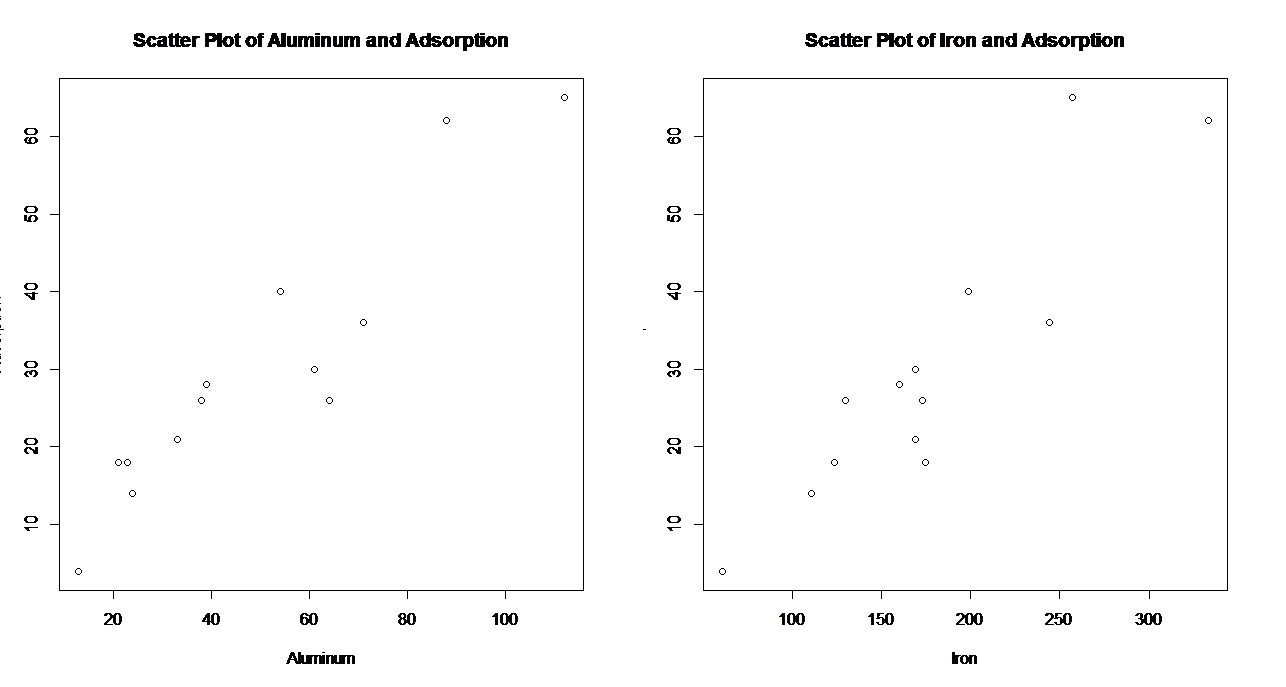
\includegraphics[scale=0.3]{scattermlr}\\
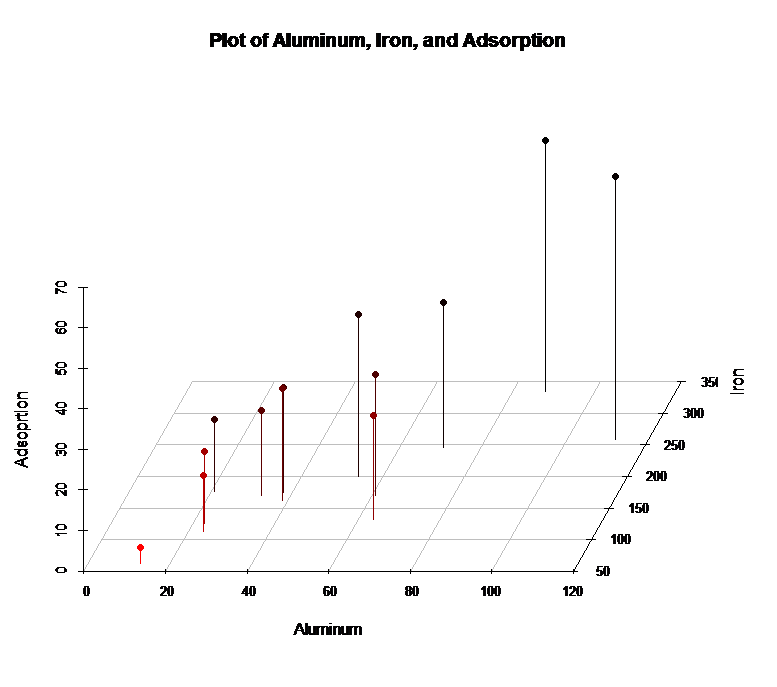
\includegraphics[scale=0.4]{scatter3dmlr}
\end{flushright}

In this case, we don`t want to find the best fitting line, but rather the best fitting \textit{plane} (the one the minimizes the squared distances between the plane and the data points). \\~\\

\begin{flushleft}
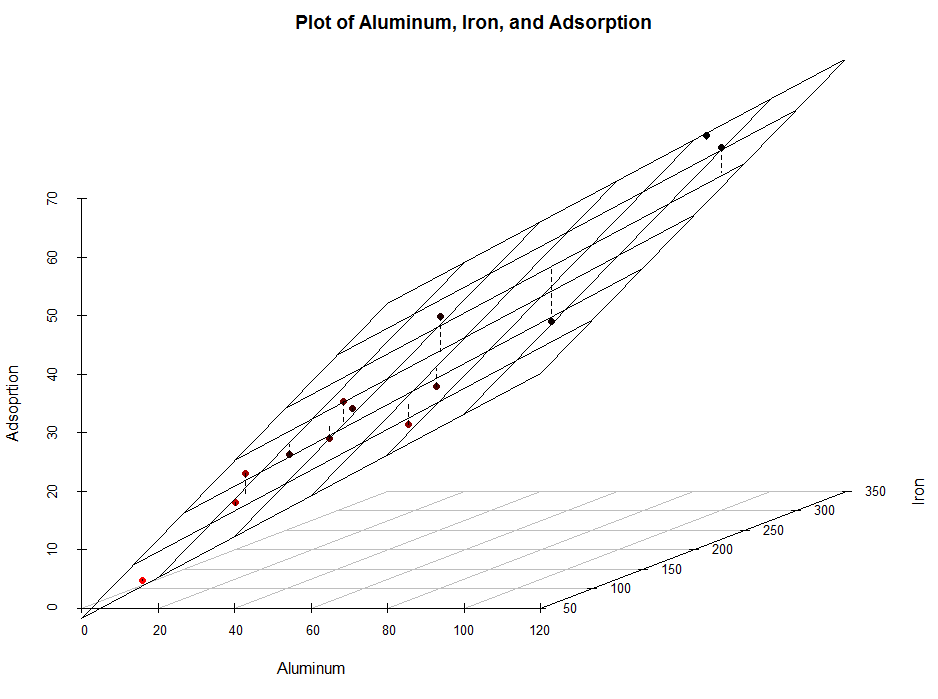
\includegraphics[scale=0.45]{adsorptionplot3d}
\end{flushleft}

\textcolor{blue}{In SLR we are testing if a `flat' line is reasonable given the data, with 2 predictors we are testing for a `flat' plane.}\\~\\

\begin{flushleft}
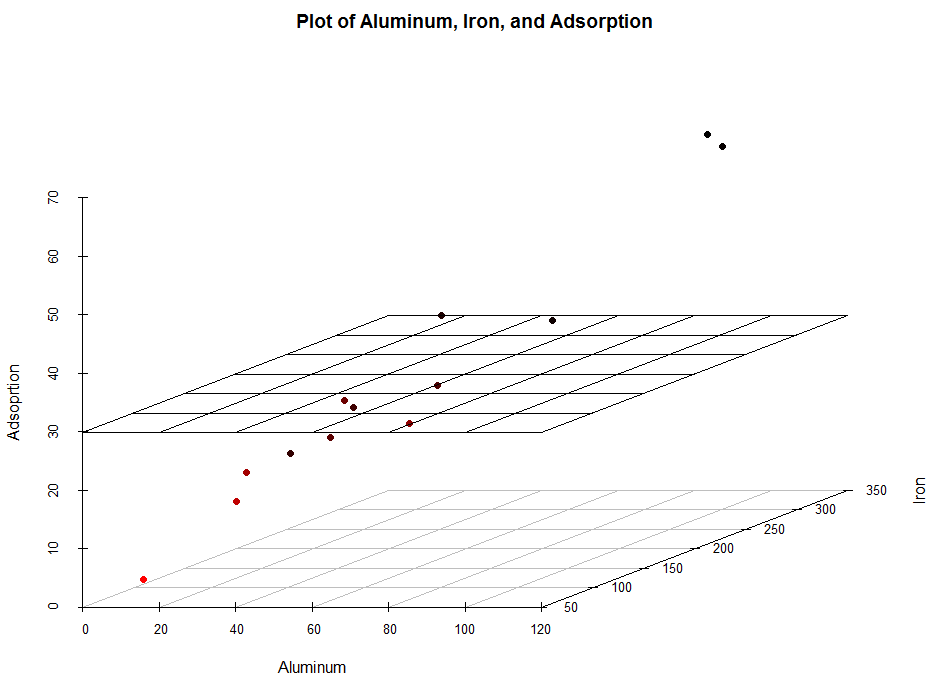
\includegraphics[scale=0.45]{adsorptionplot3dNull}
\end{flushleft}

\Large\textbf{Inferential Objective:}\large\\
Our hypothesis of interest is that at least one of our variables is useful (i.e. at least one partial slope is truly non-zero).  We can then test (called the global test)
$$H_0: \beta_1=\beta_2=0 ~~vs~~H_A: \text{ at least one is non-zero}$$
This is the hypothesis tested by the ANOVA table p-value.\\~\\

\textbf{To fit this model in SAS}
\begin{small}
\begin{verbatim}
proc reg data=adexp ; model adsorp=aluminum iron/clb; run;
\end{verbatim}
\end{small}
~\\
\begin{flushleft}
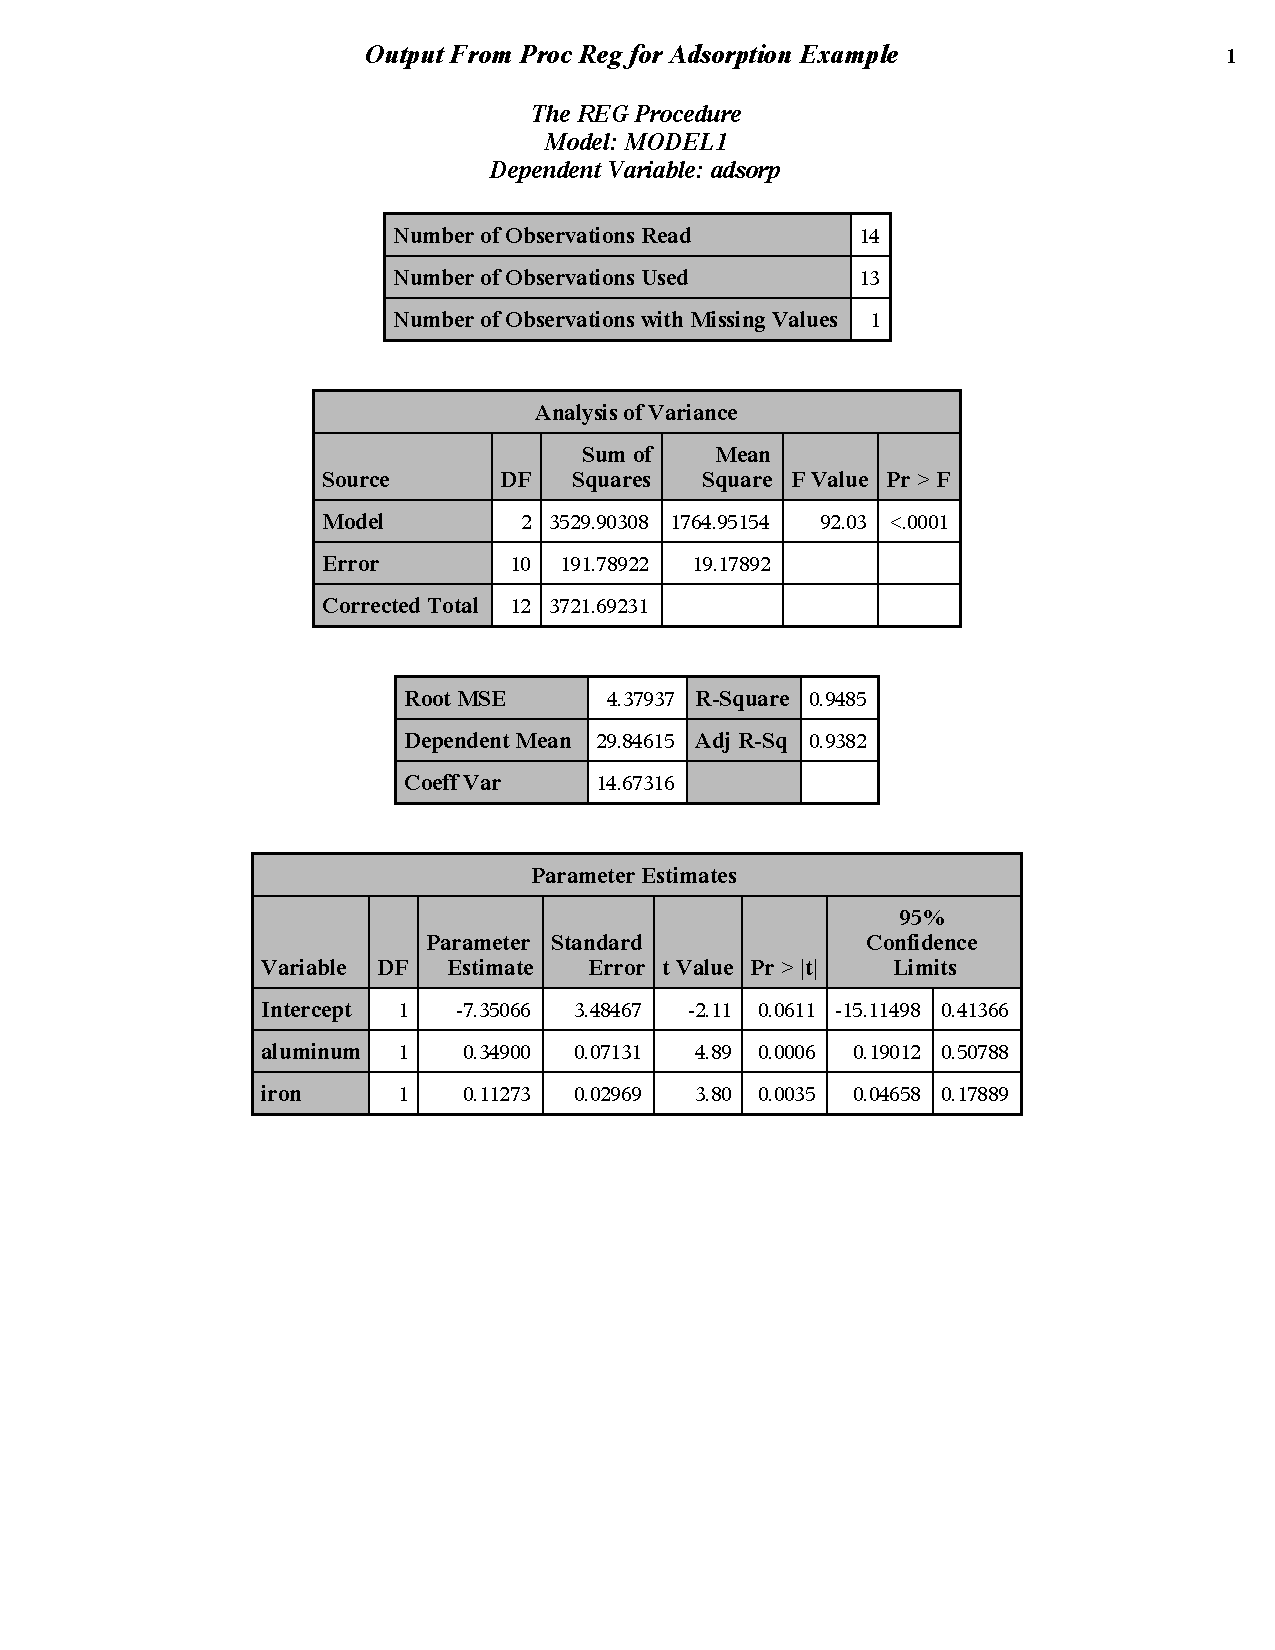
\includegraphics[page=1,scale=0.7,trim = 20mm 70mm 30mm 20mm]{mlradexp}\\
\end{flushleft}

Fitted model:
%\textcolor{red}{$$\hat{y}= \hat\beta_0 + \hat\beta_1 x_{1} + \hat\beta_2 x_{2} = -7.3507+0.3490x_1+0.1127x_2$$}
\newpage

The surface we fit can be very flexible.  All we need to do is include quadratic terms and interaction terms.\\~\\
The plots below give a number of surfaces that can be fit using two predictors when quadratic or interaction terms are included.
\begin{center}
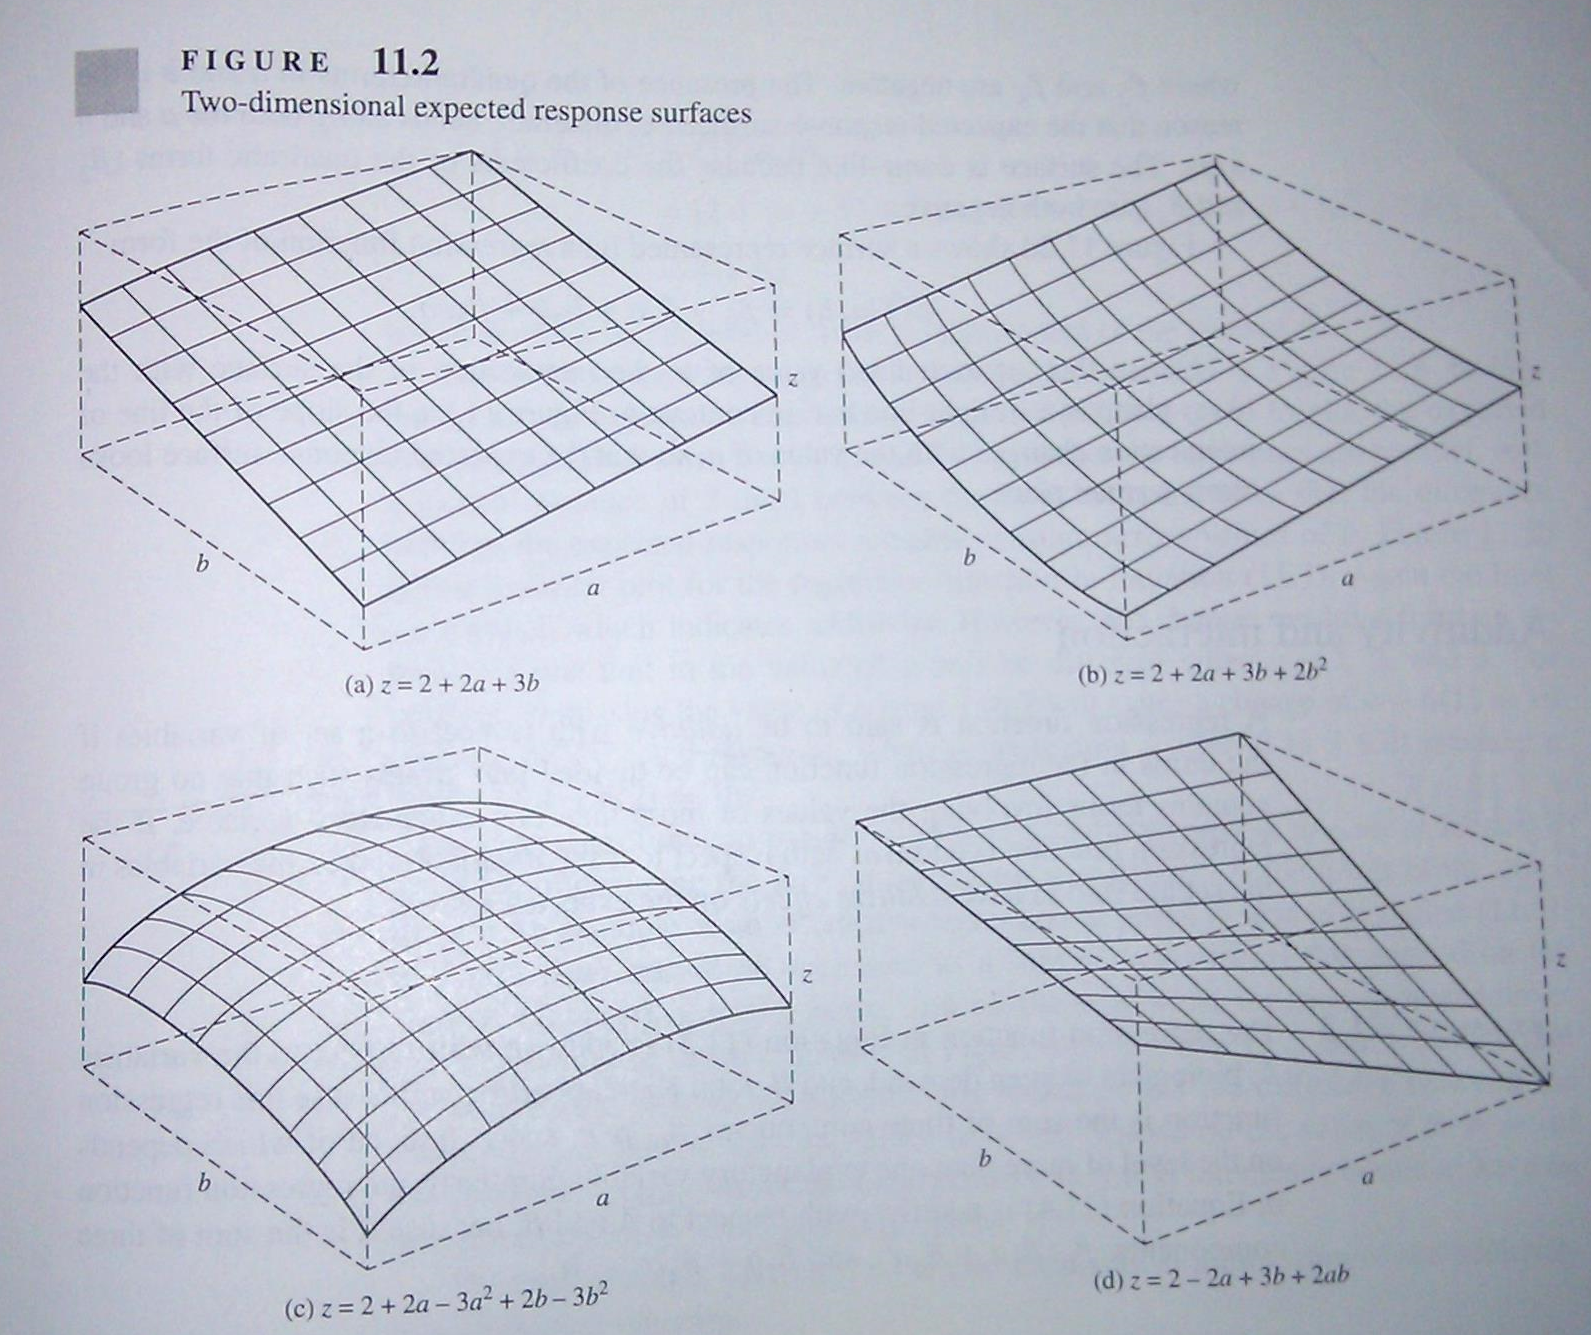
\includegraphics[scale=0.3]{surfaces}
\end{center}

A link to visualizing different surfaces:  \begin{verbatim} http://www.ats.ucla.edu/stat/sas/teach/reg_int/reg_int_cont.htm \end{verbatim}~\\~\\

These types of models are very important!  For instance, if you'd like to optimize your response over two predictors, you might fit a quadratic model in both as in the bottom left plot.\\~\\


\newpage

\Large\textbf{Interaction MLR model for two quantitative explanatory variables:}\large\\
$$Adsorption = \beta_0+\beta_1Aluminum+\beta_2Iron+\beta_3Aluminum*Iron+Experimental~Error$$
For observation $i$ we write 
$$Y_i = \beta_0 + \beta_1 x_{i1} + \beta_2 x_{i2} + \beta_3x_{i1}x_{i2}+E_{i}$$

(This surface for would be similar to the bottom right plot above.)  \\~\\

Our global test would now be 
$$H_0:\beta_1=\beta_2=\beta_3=0~~~~~vs~~~~~H_A:\mbox{ at least 1 not zero}$$
(no predictors important vs something in the model is important).\\

\textbf{To fit this model in SAS}
\begin{small}
\begin{verbatim}
proc glm data=adexp ;
model adsorp=aluminum iron aluminum*iron/solution clparm;
run;
\end{verbatim}
\end{small}

\begin{flushleft}
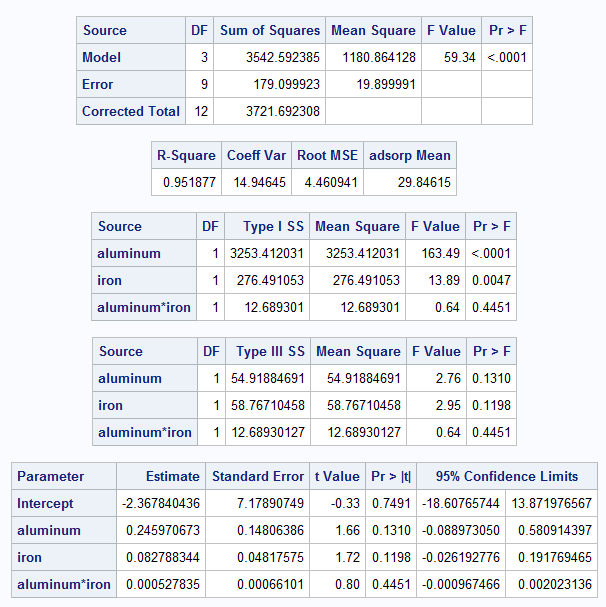
\includegraphics[scale=0.65]{adsorptioninteraction}\\
\end{flushleft}

Note:  None of the parameter estimates have significant p-values.  We'll talk about this soon.

\newpage


\Large\textbf{General MLR model for $p$ predictors $x_1, x_2,\ldots, x_p$ and response $Y$}\large\\
$$ Y_i = \beta_0 + \beta_1 x_{i1} + \beta_2 x_{i2} + \cdots + \beta_p x_{ip} + E_i$$
\textbf{Assumptions} 
\begin{itemize}
\item The true underlying relationship exists and $\mu_(x_1,...,x_p)=\beta_0 + \beta_1 x_{i1} + \cdots+\beta_p x_{ip}$.
\item Observations observed with random error $E_i$ - where $E_i\sim^{iid}~N(0,\sigma^2)$.
\end{itemize}
~\\~\\
When we fit an MLR model with $p$ different predictors we are really attempting to find the best `response surface' of degree $p$ in a $p+1$ dimensional space.  For instance,
\begin{itemize}  
\item with one predictor, we are fitting the best line in a 2-d space
\item with two predictors, we are fitting the best plane in a 3-d space.
\end{itemize}

Note: The model is written for $p$ predictors but $x_2$ could really be $x_1^2$ and $x_3$ could really be $x_1x_2$.\\~\\

\textbf{ANOVA Table}\\
Generally, the global test is
$$H_0: \beta_1=\beta_2=...=\beta_p=0 ~~vs~~H_A: \text{ at least one is non-zero}$$
Again, this is the hypothesis tested by the ANOVA table p-value.\\~\\

The ANOVA table for MLR follows the same ideas as in SLR.  \\~\\
Take the total amount of variation in the response, $SS(Tot)$, and partition it
\begin{itemize}
\item into a part due to the model, $SS(R)$
\item into a part due to experimental error, $SS(E)$.
\end{itemize}
In fact, the formulas for the sums of squares remain the same, only the degrees of freedom and the $F$-distribution used for finding the p-value change.\\~\\

The full ANOVA table for MLR is given below:\\
\begin{tabular}{|c|c|c|c|c|} \hline
Source & df & Sum of squares & Mean Square & F-Ratio \\ \hline
Regression &  p &$SS(R)$ & $MS(R)$ & $MS(R)/MS(E)$ \\
Error & $n-p-1$ & $SS(E)$ &$MS(E)$ &  \\
Total & $n-1$ & $SS(Tot)$ & &  \\ \hline
\end{tabular}

\newpage

\Large\textbf{Fitting the Model}\large\\
Regression parameters ($\beta$'s) estimated using least squares as in SLR
$$ min_{\hat{\beta}'s} SS(E)$$
where 
$$SS(E) = \sum_{i=1}^n (y_i-\hat{y}_i)^2=\sum_{i=1}^n (y_i - \hat{\beta}_0 - \hat{\beta}_1 x_{i1} - \cdots - \hat{\beta}_p x_{ip})^2$$
and our estimate for the error variance is similarly defined as
$$\hat\sigma^2 = MS(E)=\frac{SS(E)}{df_E}=\frac{\sum_{i=1}^n (y_i-\hat{y}_i)^2}{n-p-1}$$


\textcolor{blue}{There are formulas for the estimates of our regression parameters, however, they are cumbersome to write out the way we have been doing. \\~\\
We will also want to make inference, which implies that we will need to know about the variability of the estimates. \\~\\
It will be much easier to write all of these things out using matrix notation.}\\~\\

\Large\textbf{Interpretations of regression parameters:}\large
\begin{itemize}
\item $\sigma^2$ = unknown \textbf{error variance} parameter (measure of variability due to experimental error). 
\item $\beta_0, \beta_1, \ldots, \beta_p$ are $p+1$ unknown regression parameters:
	\begin{itemize}
	\item $\beta_0$ = average response when $x_1 = x_2 = \ldots = x_p =0$\\~\\~\\~\\~\\
	%\textcolor{red}{$\mu_{x_1,...,x_p}=\beta_0+\beta_1x_{1}+...+\beta_px_{p}$
	%$\rightarrow \mu_{0,...,0}=\beta_0$}
	\item $\beta_i$ is called the \textbf{partial slope} for $x_i$. 
	\begin{itemize}
	\item For the additive model linear with unique $x's$, $\beta_i$ represents the estimated change in mean of $Y$ per unit increase in $x_i$ \textbf{with all other independent variables held fixed}. 
%	\textcolor{red}{\mu_{x_1,...,x_{i}+1,...,x_p}-\mu_{x_1,...,x_{i},...,x_p}=\beta_i}
\end{itemize}
\end{itemize}
\end{itemize}

\newpage

\Large\textbf{Inference for regression parameters:}\large\\
Similar to the SLR case, we still use t-tests to test our hypotheses of interest
$$H_0:\beta_i=0~~~~~~vs~~~~~H_A:\beta_i\neq 0$$
Test Statistic:
$$T=\frac{\hat{\beta}_i}{\hat{SE}(\hat{\beta}_i)}\sim^{H_0} t_{n-p-1}$$
To make a conclusion we use
$$RR=\left\{t_{obs}:|t_{obs}|>t_{\alpha/2,n-p-1}\right\}$$
or
$$p-value=2*P(T_{n-p-1}>|t_{obs}|)$$~\\~\\

\textcolor{blue}{To actually know about the SE, to find a CI for $\mu(x_1,...,x_p)$, or to find a PI for a future observation at $x_1,...,x_p$ we will need to look at the matrix formulation of this model.}

\newpage

\Large\textbf{Very brief matrix review:}\large\\
Note: Capital boldface letters are usually used for matrices and boldface lower case letters are usually used for vectors (matrices where the number of rows or the number of columns is 1).\\~\\
\textbf{Matrices} - rectangular arrays of numbers that have a great many uses.  Some matrices, (with {\em dimension} in parentheses):
\[
\begin{array}{cccc}
\textbf{A}&=&\left(\begin{array}{cc} 7 & 5 \\ 5 & 2 \\ 3 & 2 \end{array}\right)  & (3 \times 2) \\
\textbf{B}&=&\left(\begin{array}{ccc} 4 & 2 & 1 \\ 3 & 1 & 1 \end{array}\right)  & (2 \times 3)  \\
\textbf{C}&=&\left(\begin{array}{cc} 1 & 1 \\ -1 & 1 \end{array}\right) & (2 \times 2) \\
\textbf{I}_2&=&\left(\begin{array}{cc} 1 & 0 \\ 0 & 1 \end{array}\right) & (2 \times 2)
\end{array}
\]
~\\~\\
One of the most important uses of matrices is to represent systems of equations.  For instance say we take a subset of the Adsorption data and look at the SLR model between adsorption and aluminum ($x$):
$$Y_1=\beta_0+\beta_1*x_1+E_1$$
$$Y_2=\beta_0+\beta_1*x_2+E_2$$
$$Y_3=\beta_0+\beta_1*x_3+E_3$$
We can write this in matrix form as
$$\textbf{y}=\left(\begin{array}{c}Y_1 \\ Y_2\\ Y_3\end{array}\right)~~~~~~~~\textbf{X}=\left(\begin{array}{cc} 1 & x_1\\ 1 & x_2 \\ 1 & x_3\end{array}\right)~~~~~~~\boldsymbol{\beta}=\left(\begin{array}{c}\beta_0\\\beta_1\end{array}\right)~~~~~\textbf{e}=\left(\begin{array}{c} E_1\\E_2\\E_3\end{array}\right)$$
The system is now
$$\textbf{y}=\textbf{X}\boldsymbol{\beta}+\textbf{e}$$

\newpage

\textbf{Recall Some Basic Matrix Operations}
\begin{enumerate}
\item Dimension of a matrix = \# of rows $\times$ \# of columns

\item Multiplication - requires {\em conformability} of matrices\\
(i.e. for \textbf{AB} to be defined - \# of columns of A must be the same as the \# of rows of B)\\~\\
\textbf{AB} matrix has $(i,j)$ element given by `dot-product' of $i^{th}$ row of $\textbf{A}$, $j^{th}$ column of $\textbf{B}$:
\[ 
\begin{array}{ccc}
\textbf{AB} & = & 
\left(\begin{array}{cc} 7 & 5 \\ 5 & 2 \\ 3 & 2 \end{array}\right)  
\left(\begin{array}{ccc} 4 & 2 & 1 \\ 3 & 1 & 1 \end{array}\right)  
\\
& & \\
& & \\
& = & \left(\begin{array}{ccc} 
7 \cdot 4 + 5 \cdot 3, & 
7 \cdot 2 + 5 \cdot 1, & 
7 \cdot 1 + 5 \cdot 1 \\
5 \cdot 4 + 2 \cdot 3, & 
5 \cdot 2 + 2 \cdot 1, & 
5 \cdot 1 + 2 \cdot 1 \\
3 \cdot 4 + 2 \cdot 3, & 
3 \cdot 2 + 2 \cdot 1, & 
3 \cdot 1 + 2 \cdot 1 \end{array}\right) \\
& & \\
& & \\
& = & \left(\begin{array}{ccc} 43 & 19 & 12 \\ 26 & 12 & 7 \\ 18 & 8 & 5 \end{array}\right) \end{array}
\] 
Note: Unlike scalar multiplication, the product $\textbf{DE}$ is not usually equal to $\textbf{ED}$. \\~\\~\\

For our system, we have\\~\\
$\textbf{X}\boldsymbol{\beta}=$\\~\\~\\~\\~\\
%\textcolor{red}{\left(\begin{array}{cc} 1 & x_1\\ 1 & x_2 \\ 1 & x_3\end{array}\right)\left(\begin{array}{c}\beta_0\\\beta_1\end{array}\right)=\left(\begin{array}{c}\beta_0+\beta_1x_1\\\beta_0+\beta_1x_2\\\beta_0+\beta_1x_3\end{array}\right)}$\\~\\~\\

Note: A special matrix is called the \textbf{Identity Matrix} and is denoted by $\textbf{I}$.  It is a {\em square},
{\em symmetric}, and {\em diagonal} with $1's$ along the diagonal and $0's$
elsewhere:
$$\textbf{I}_3 = \left(\begin{array}{ccc} 1 & 0 & 0 \\ 0 & 1 & 0 \\ 0 & 0 & 1 \end{array}\right) $$
Multiplication of any (conformable) matrix $\textbf{M}$ by $\textbf{I}$ gives $\textbf{M}$:
$\textbf{AI}_2 = \textbf{A} = \textbf{I}_3 \textbf{A}$
~\\~\\

\item Addition - performed element-wise, matrices must have same {\em dimension} (same \# of rows and columns)
\[ 
\textbf{C} + \textbf{I}_2 = 
\left(\begin{array}{cc} 1 + 1 & 1 + 0 \\ -1 + 0  & 1 + 1 \end{array}\right) 
=
\left(\begin{array}{cc} 2 & 1 \\ -1 & 2 \end{array}\right) \ \ (2 \times 2)
\]
~\\~\\
Subtraction, same deal
\[ 
\textbf{C} - \textbf{I}_2 = \left(\begin{array}{cc} 0 & 1 \\ -1 & 0 \end{array}\right) \ \ (2 \times 2)
\]
~\\~\\

For our system we have \\~\\
$\textbf{X}\boldsymbol{\beta}+\textbf{E}=$\\~\\~\\~\\~\\~\\
%\textcolor{red}{\left(\begin{array}{c}\beta_0+\beta_1x_1\\\beta_0+\beta_1x_2\\\beta_0+\beta_1x_3\end{array}\right)+\left(\begin{array}{c}E_1\\E_2\\E_3\end{array}\right)=\left(\begin{array}{c}\beta_0+\beta_1x_1+E_1\\\beta_0+\beta_1x_2+E_2\\\beta_0+\beta_1x_3+E_3\end{array}\right)}$\\~\\~\\
Thus, we have represented our system of equations using these matrices!
$$\textbf{y}=\textbf{X}\boldsymbol{\beta}+\textbf{E}$$~\\

Other properties we need:
\item Inverse -  The {\em inverse} $\textbf{M}^{-1}$ of a {\em square} ($r \times r$) matrix $\textbf{M}$,
if it exists, satisfies $\textbf{MM}^{-1}=\textbf{I}_r$ (similar to the reciprocal of real number giving us 1).\\
 A square matrix with an inverse is called {\em non-singular}.\\~\\
Inversion can be computationally challenging, but not for
$(2 \times 2)$ case:
$$ \left(\begin{array}{cc} a & b \\ c & d \end{array}\right) = 
\frac{1}{ad-bc}
\left(\begin{array}{cc} d & -b \\ -c & a \end{array}\right) $$
Find $\textbf{C}^{-1}$.
$$\textbf{C}^{-1} = \frac{1}{2}\left(\begin{array}{cc} 1 & -1 \\ 1 & 1\end{array}\right)=\left(\begin{array}{cc} 1/2 & -1/2 \\ 1/2 & 1/2\end{array}\right)$$~\\
Now 
$$\textbf{C}\textbf{C}^{-1}=\left(\begin{array}{cc} 1 & 1 \\ -1 & 1 \end{array}\right)\left(\begin{array}{cc} 1/2 & -1/2 \\ 1/2 & 1/2\end{array}\right)=\left(\begin{array}{cc} 1 & 0 \\ 0 & 1\end{array}\right)$$

%The {\em rank} of a matrix is equal to the number of {\em linearly independent}
%rows or columns of the matrix.  Vectors $\textbf{x}_1,\textbf{x}_2,\ldots,\textbf{x}_n$ are linearly independent
%if $\sum_i a_i \textbf{x}_i = 0$ implies $a_1=a_2=\cdots=a_n=0$.

\item Transposition - swap rows for columns, columns for rows (turn matrix on its side):
\[
t(\textbf{A}) = \textbf{A}` = \textbf{A}^{T} = 
\left(\begin{array}{ccc} 7 & 5 & 3 \\ 5 & 2 & 2 \end{array}\right) \ \ \mbox{``transpose of $\textbf{A}$"}
\]
\end{enumerate}
~\\

\Large How can we use this matrix representation?\large\\
Using our example, say we've observed the first three observations:
$$4=\beta_0+\beta_{1}13$$
$$18=\beta_0+\beta_{1}21$$
$$14=\beta_0+\beta_{1}24$$~\\
Now our goal is to estimate the $\beta$ parameters here.  We can use matrices to represent this scenario!
$$\textbf{y}=\left(\begin{array}{c}4 \\ 18\\ 14\end{array}\right)~~~~~~~~\textbf{X}=\left(\begin{array}{cc} 1 & 13\\ 1 & 21 \\ 1 & 24\end{array}\right)~~~~~~~\boldsymbol{\beta}=\left(\begin{array}{c}\beta_0\\\beta_1\end{array}\right)$$
~\\~\\
The system is now
$$\textbf{y}=\textbf{X}\boldsymbol{\beta}$$
and we want to find the optimal $\boldsymbol{\beta}$ - by optimal the $\boldsymbol{\beta}$ that minimizes 
$$SS(E) = (\textbf{y}-\textbf{X}\boldsymbol{\beta})^T(\textbf{y}-\textbf{X}\boldsymbol{\beta}).$$~\\~\\
We could optimize $\boldsymbol{\beta}$ via calculus yielding the `normal equations'
$$\textbf{X}^{T}\textbf{X}\boldsymbol{\beta}=\textbf{X}^{T}\textbf{y}$$
and our estimates written as 
$$\boldsymbol{\hat{\beta}}=\left(\textbf{X}^{T}\textbf{X}\right)^{-1}\textbf{X}^{T}\textbf{y}$$~\\~\\

\newpage

If we have a random vector (just like a random variable but in vector form, i.e. components yield numeric answers that are random), call it $\textbf{Y}$ and a constant vector, call it \textbf{a}, then\\~\\~\\~\\~\\~\\~\\~\\~\\~\\~\\
%\textcolor{red}{$$E(\textbf{a}^{T}\textbf{Y}) = \textbf{a}^{T}E(\textbf{Y})$$
%$$\Var(\textbf{a}^{T}\textbf{Y}) = \textbf{a}^{T}\Var(\textbf{Y})\textbf{a}$$}~\\~\\

Now, when we want to make inference about a given $\beta$ element (or a combination of them) we can use Expected Value and Variance properties of this matrix.
\begin{eqnarray*}
E(\boldsymbol{\hat{\beta}})& = &E((\textbf{X}^{T}\textbf{X})^{-1} \textbf{X}^{T}\textbf{Y})\\
&=&(\textbf{X}^{T}\textbf{X})^{-1} \textbf{X}^{T}E(\textbf{Y})\\
&= &(\textbf{X}^{T}\textbf{X})^{-1} \textbf{X}^{T}\textbf{X}\boldsymbol{\beta}=\boldsymbol{\beta}
\end{eqnarray*}
~\\
\begin{eqnarray*}
Var(\boldsymbol{\hat{\beta}})&=&\Var((\textbf{X}^{T}\textbf{X})^{-1} \textbf{X}^{T}\textbf{Y})\\
&=&(\textbf{X}^{T}\textbf{X})^{-1} \textbf{X}^{T}Var(\textbf{Y})\textbf{X}(\textbf{X}^{T}\textbf{X})^{-1}\\
&=&(\textbf{X}^{T}\textbf{X})^{-1} \textbf{X}^{T}\sigma^2\textbf{I}_{n}\textbf{X}(\textbf{X}^{T}\textbf{X})^{-1}\\
&=&\sigma^2 (\textbf{X}^{T}\textbf{X})^{-1}\textbf{X}^{T}\textbf{X}(\textbf{X}^{T}\textbf{X})^{-1}\\
&=&\sigma^2(\textbf{X}^{T}\textbf{X})^{-1}=\boldsymbol{\Sigma}
\end{eqnarray*}

The variance involves the true error variance so we will estimate it by
$$\widehat{\boldsymbol{\Sigma}}=\widehat{\Var}(\hat{\boldsymbol{\beta}})  =  MS(E)(\textbf{X}^{T}\textbf{X})^{-1}$$
~\\~\\

\textcolor{blue}{Understanding matrices if very important as this is how we will look at our models for the rest of the MLR section and the GLM section.  Also, SAS and other statistical programs use matrices in their calculations and in their output.}

\newpage

\Large \textbf{General Matrix formulation of MLR}\large\\
\begin{center}
$\textbf{Y} = \textbf{X}\boldsymbol{\beta} + \textbf{E}$
\end{center}
All of the response RVs are placed into the \textbf{response vector}:
$$\textbf{Y}=\left(\begin{array}{c}
Y_1\\
Y_2\\
\vdots\\
Y_n\\
\end{array}\right)$$
For observation $i$ we can group all of the explanatory variables into a vector
$$\textbf{x}_{i} = (1,x_{i1},x_{i2},x_{i3},\ldots,x_{ip}).$$~\\
The 1 in the first spot of the vector is for the intercept.  If we `stack' these row vectors on top of each other we can make a matrix called the \textbf{design matrix}:
$$
\textbf{X}=\left(\begin{array}{ccccc}
1  &  x_{11}  &   x_{12} & \ldots & x_{1p} \\
1  &  x_{21}  &   x_{22} & \ldots & x_{2p} \\
\vdots &\vdots &\vdots &\vdots &\vdots \\ 
1  &  x_{n1}  &   x_{n2} & \ldots & x_{np} \\
\end{array}\right)$$

%\textcolor{red}{Remember 1st subscript is the observation number and the second subscript tells us which explanatory variable we are using.}\\~\\

We also form a column vector corresponding to the regression parameters, called the \textbf{`beta vector'}:
$$\boldsymbol{\beta}=\left(\begin{array}{c}
\beta_0\\
\beta_1\\
\vdots\\
\beta_p\\
\end{array}\right)$$

and a column vector for the error terms, called the \textbf{error vector}:
$$\textbf{E}=\left(\begin{array}{c}
E_1\\
E_2\\
\vdots\\
E_n\\
\end{array}\right)$$


Now we can see that our MLR model (a system of $n$ equations with $p+1$ unknowns) 
\begin{eqnarray*}
Y_1 & = & \beta_0 + \beta_1 x_{11} + \beta_2 x_{12}+ \cdots + \beta_p x_{1p} + E_1 \\
Y_2 & = & \beta_0 + \beta_1 x_{21} + \beta_2 x_{22}+ \cdots + \beta_p x_{2p} + E_2 \\
\vdots & = & \vdots \\
Y_n & = & \beta_0 + \beta_1 x_{n1} + \beta_2 x_{n2}+ \cdots + \beta_p x_{np} + E_n
\end{eqnarray*}
can be easily rewritten as
\begin{center}
$\textbf{y} = \textbf{X}\boldsymbol{\beta} + \textbf{E}$
\end{center}

\newpage

Our assumptions on the errors can now be specified as 
$$\textbf{E}\sim N_n(\boldsymbol{0},\sigma^2 \textbf{I}_{n}) \mbox{   (multivariate normal distribution)}$$
where $\sigma^2 \textbf{I}_{n}$ is called the variance-covariance matrix of the errors:\\~\\~\\~\\~\\~\\~\\~\\~\\~\\~\\
%\textcolor{red}{$$
%Var(\textbf{E})=\left(\begin{array}{cccc}
%\sigma^2  &  0  &   \ldots & 0 \\
%0  &  \sigma^2  &   \ldots & 0 \\
%\vdots &\vdots &\vdots &\vdots  \\ 
%0  &  0  &  \ldots & \sigma^2 \\
%\end{array}\right)$$}~\\~\\


The diagonals of the matrix give the variances for the $E_i$`s ($Var(E_1), Var(E_2), \ldots, Var(E_n)$) and the off-diagonals (say row $i$ column $j$) give the covariances between $E_i$`s and the $E_j$`s ($Cov(E_i, E_j)$).  \\~\\
As the off-diagonals are all 0, our errors are uncorrelated (which for the multivariate normal distribution implies independence).\\~\\

Later in the semester, we will consider cases (such as block designs and split plots) where this variance-covariance matrix will not be diagonal.\\~\\~\\

Note: Similarly, we have the variance-covariance matrix of our $\boldsymbol{\beta}$ vector:\\~\\

$$\boldsymbol{\Sigma}=Var(\boldsymbol{\hat{\beta}})=\sigma^2\left(\textbf{X}^{T}\textbf{X}\right)^{-1}=\left(\begin{array}{ccccc} Var(\hat{\beta}_0) & Cov(\hat{\beta}_0,\hat{\beta}_1) & Cov(\hat{\beta}_0,\hat{\beta}_2) & \cdots & Cov(\hat{\beta}_0,\hat{\beta}_p)\\
 & Var(\hat{\beta}_1) & Cov(\hat{\beta}_1,\hat{\beta}_2) & \cdots & Cov(\hat{\beta}_1,\hat{\beta}_p)\\
 & & Var(\hat{\beta}_2) & \cdots & Cov(\hat{\beta}_2,\hat{\beta}_p)\\
 &  &  & \vdots & \vdots\\
 & & & & Var(\hat{\beta}_p)\end{array}\right)$$

\newpage

Let`s look at some of these quantities for our adsorption example.  We have $n=13$ and $p=2$.
\begin{center}
\begin{tabular}{ccc}
\textbf{y}=$\left(\begin{array}{c} 4 \\18\\14\\18\\26\\26\\21\\30\\28\\36\\65\\62\\40\\\end{array}\right)$ &
\textbf{X}=$\left(\begin{array}{ccc}1&13& 61\\1&21&175\\1&24&111\\1&23&124\\1&64&130\\1&38&173\\1&33&169\\1&61&169\\1&39&160\\1&71&244\\1&112&257\\1&88&333\\1&54&199\\\end{array}\right)$&
$\boldsymbol{\beta}$=$\left(\begin{array}{c} \beta_0 \\\beta_1\\\beta_2\\\end{array}\right)$ 
\end{tabular}
\end{center}
~\\~\\
$$\textbf{X}'\textbf{X} = \left(\begin{array}{ccc} 13&641&2305\\ 641&41831 & 133162\\ 2305&133162 &467669\\\end{array}\right)$$
~\\~\\
$$(\textbf{X}'\textbf{X})^{-1} = \left(\begin{array}{ccc} 0.633138 &0.002477&-0.003826\\ 0.002477 & 0.000265 & -0.000088\\ -0.003826 &-0.000088 &0.000046 \\\end{array}\right)$$
~\\~\\
$$\hat{\boldsymbol{\beta}}= (\textbf{X}'\textbf{X})^{-1} \textbf{X}'\textbf{Y} = \left(\begin{array}{cc} -7.3507\\  0.3490\\ 0.1127\\\end{array}\right)$$
~\\~\\
$$\hat{\boldsymbol{\Sigma}}=MS(E)(\textbf{X}'\textbf{X})^{-1} = \left(\begin{array}{ccc}
 12.14294&  0.04750& -0.07337\\
 0.04750  &0.00508 &-0.00168\\
 -0.07337 &-0.00168&  0.00088\\
\end{array}\right)$$

\newpage

The parameter estimates and the variance-covariance matrix are very useful for making inference about our intercept and partial slope parameters (done very similary to SLR).  Let`s use the above to find the following
\begin{enumerate}
\item What is the fitted equation?\\~\\~\\~\\
%\textcolor{red}{\\$\hat{\beta}_0+\hat{\beta}_1x_1+\hat{\beta}_2x_2=-7.3507+0.3490x_1+0.1127x_2$}
\item What is the estimate for $\beta_2$?  What is its interpretation?\\~\\~\\~\\~\\~\\
%\textcolor{red}{\\$\hat\beta_2 =0.1127$, which represents the estimated change in adsorption for a one unit increase in extractable iron while holding the amount of extractable aluminum constant.}
\item What is the estimated standard error of $\hat\beta_2$, $\hat{SE}(\hat\beta_2)$?  \\~\\~\\~\\
%\textcolor{red}{\\$\sqrt{0.00088}=0.0297$ (square root of (3,3) element of $\widehat{\boldsymbol{\Sigma}}$)}
\item Conduct a test to determine if $\beta_2=0$ is plausible (once accounting for $X_1$).  This is a test for the importance of extractable iron once the relationship between extractable aluminum and adsorption index is accounted for (called a type III test, more on this later).  Note: $t_{0.025, 10}=2.228$\\
%\textcolor{red}{\\$H_0: \beta_2=0 ~~ vs ~~ H_A: \beta_2\ne 0$, T-statistic: $t=(\hat\beta_2 - 0)/SE(\hat\beta_2) = 0.1127/0.0297 = 3.795$ \\
%Since our observed test statistic is greater than 2.228, we reject $H_0$ in favor of $H_A$, that is, at the 5\% significance level, extractable iron has a significant linear association with adsorption (even after accounting for extractable aluminum).}
\end{enumerate}

\newpage

\Large \textbf{Fitted Values and Residuals}\large\\
The predicted values can be written as
$$\hat{\textbf{y}} = \textbf{X} \hat{\boldsymbol{\beta}} = \textbf{X} (\textbf{X}'\textbf{X})^{-1} \textbf{X}'\textbf{y} = \textbf{H} \textbf{y} $$
\begin{itemize}
\item $\hat{\textbf{y}}$ is called the vector of \underline{fitted} or \underline{predicted values}
\item $\textbf{H}=\textbf{X}(\textbf{X}'\textbf{X})^{-1}\textbf{X}$ is called the \underline{hat matrix} as it `places' the hat on $\textbf{y}$
\end{itemize}
~\\~\\~\\
The residuals as
$$\textbf{e}  =  \textbf{y}-\hat{\textbf{y}}  =  \textbf{y} - \textbf{X}\hat{\boldsymbol{\beta}} =  (\textbf{I}-\textbf{H}) \textbf{y}$$~\\

We are still using least squares to select the parameters, which can be written as the minimum of:
$$SS(E) = \sum_{i=1}^{n}(obs_i-pred_i)^2=\sum_{i=1}^n(y_i-\hat{y}_i)^2=\sum_{i=1}^n (y_i - \beta_0 - \beta_1 x_{i1} - \cdots - \beta_p x_{ip})^2=\textbf{e}'\textbf{e}$$

$$\begin{array}{cc}
\hat{\textbf{y}} = \textbf{X}\hat{\boldsymbol{\beta}} = \left(\begin{array}{c}4.0610\\19.7008\\13.5350\\14.6511\\29.6363\\25.4084\\23.2126\\32.9846\\24.2923\\44.9271\\60.7012\\60.8904\\33.9226\\\end{array}\right) & 
\textbf{e}=\boldsymbol{y}-\hat{\boldsymbol{y}}= \left(\begin{array}{c} 4 \\18\\14\\18\\26\\26\\21\\30\\28\\36\\65\\62\\40\\\end{array}\right)-\left(\begin{array}{c}4.0610\\19.7008\\13.5350\\14.6511\\29.6363\\25.4084\\23.2126\\32.9846\\24.2923\\44.9271\\60.7012\\60.8904\\33.9226\\\end{array}\right)= \left(\begin{array}{c}-0.0610\\-1.7008\\0.4650\\3.3489\\-3.6363\\0.5916\\-2.2126\\-2.9846\\3.7077\\-8.9271\\4.2988\\1.1096\\6.0774\\\end{array}\right)
\end{array}
$$

$$SS(E) = \textbf{e}'\textbf{e} = 191.7897$$
$$\hat{\sigma}^2=MS(E) = SS(E)/(n-p-1) = 191.7897/10 = 19.17897 $$

\newpage

\Large \textbf{Inference about a mean or a future value}\large\\

To make inference about some linear combination of $\hat\beta$`s such as 
$$\hat{\mu}(x_1,x_2,...x_p)=\hat{\beta}_{0}+\hat{\beta}_{1}x_{1}+\hat{\beta}_{2}x_{2}+\ldots+\hat{\beta}_{p}x_{p}$$
we can again use matrix/vector notation to make things easy. \\~\\
Define 
$$\textbf{a}=\left(\begin{array}{c}1 \\x_1\\x_2\\...\\x_p\end{array}\right)$$
The mean above can be rewritten as
$$(1~~x_{1}~~x_{2}~~\ldots~~x_{p})\hat{\boldsymbol{\beta}}=\textbf{a}^{T}\hat{\boldsymbol{\beta}}$$
Then we have the point estimate of
$$E(\textbf{a}^{T}\hat{\boldsymbol{\beta}}) = \textbf{a}^{T}\boldsymbol{\beta}$$
the measure of variability is 
$$\Var(\textbf{a}^{T}\hat{\boldsymbol{\beta}}) = \textbf{a}^{T}\boldsymbol{\Sigma}\textbf{a}$$
estimated as
$$\widehat{\Var}(\textbf{a}^{T}\hat{\boldsymbol{\beta}}) = \textbf{a}^{T}\widehat{\boldsymbol{\Sigma}}\textbf{a}$$
Now we can use the t-distribution (n-p-1 df) to perform Hypothesis Tests and form Confidence Intervals very similar to the SLR case.\\~\\~\\
If we want the variance of a future observation, we just add $\sigma^2$ to the variance (and thus add $MS(E)$ to the estimated variance).\\~\\

\textcolor{blue}{Note we are making the assumption that $\textbf{X}^{T}\textbf{X}$ matrix has an inverse.  This is true if $\textbf{X}$ is full `rank'.  If this is not true, generalized inverses can be used, but we won`t worry about any of that.}\\~\\

\newpage

\begin{enumerate}
\item Estimate the mean adsorption index for soil with extractable aluminum = 100 and extractable iron = 150.  \\~\\~\\~\\~\\
%\textcolor{red}{\\Unknown population mean: $\theta=\beta_0+\beta_1(100) +\beta_1(150)$ \\
%Estimate : $\hat\theta=(1,100,150)* \hat\beta = 44.454$}
\item Report a standard error for the estimate above.\\~\\~\\~\\~\\~\\
%\textcolor{red}{\\To find the standard error, find the variance and take the square root:
%$$\Var((1,100,150) * \hat{\boldsymbol{\beta}}) = (1,100,150)\Var(\hat{\boldsymbol{\beta}}) (1,100,150)'$$
%estimated as
%$$= (1,100,150)\widehat{\boldsymbol{\Sigma}} (1,100,150)'=19.832$$
%Which implies $SE(\hat\theta) = \sqrt{19.832}=4.453$.}
\item Find and interpret a $95\%$ confidence interval for the population of ALL soil with extractable aluminum = 100 and extractable iron = 150.  Note: $t_{0.025, 10}=2.228$\\~\\~\\~\\~\\~\\~\\~\\~\\
%\textcolor{red}{\\
%We are 95\% confident that the true mean adsorption index among the population of ALL soil with extractable aluminum = 100 and extractable iron = 150 is between 
%$$(44.454-2.228(4.453), 44.454-2.228(4.453)) = (34.533, 54.375)$$}
\item Find a 95\% prediction interval for a future observation with extractable aluminum = 100 and extractable iron = 150.  \\
%\textcolor{red}{\\
%The variance of a future value is $Var(\hat{\mu}(100,150))+Var(E_{new})$ which is estimated as 19.832+19.17897=39.01097.  \\
%The estimated SE is the square root $ = 6.2459$.  \\
%Therefore, we are 95\% confident that a future absorption index for soil with extractable aluminum = 100 and extractable iron  150 is between 
%$$(44.454-2.228(6.2459), 44.454-2.228(6.2459)) = (30.538, 58.370)$$}
\end{enumerate}


\newpage

\Large\textbf{How to get these intervals in SAS?}\large\\
The following code will produce output appropriate for analysis: (more practice with this in lab)
\begin{small}
\begin{verbatim}
data newad;
input adsorp aluminum iron;
datalines;
. 100 150
;

proc datasets;
append base=adexp data=newad;
run;

proc glm data=adexp plots=all;
* can only run one of clm or cli at once;
model adsorp=aluminum iron/solution clparm clm;
*model adsorp=aluminum iron/solution clparm cli;
run;
\end{verbatim}
\end{small}

\begin{flushleft}
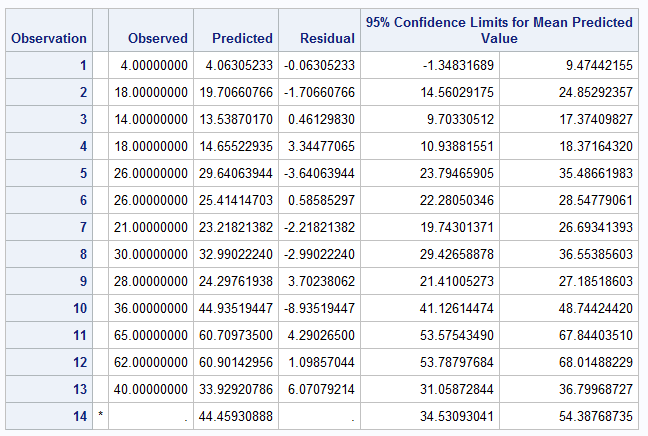
\includegraphics[scale=0.7]{adsorptionCIPI}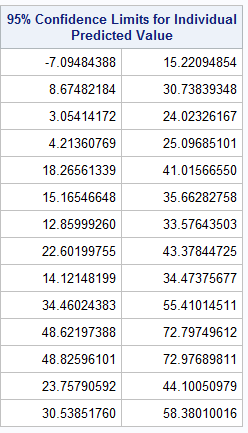
\includegraphics[scale=0.7]{adsorptionPI}\\
\end{flushleft}

\begin{flushright}
\includegraphics[page=2,scale=0.55,trim = 20mm 60mm 20mm 20mm]{mlradexp}
\\
\includegraphics[page=3,scale=0.4,trim = 20mm 120mm 20mm 20mm]{mlradexp}
\end{flushright}

\newpage

\Large\textbf{Model Selection Ideas and Methods}\large\\

\textcolor{blue}{As a researcher, there will often be some models that you want to fit with preselected variables.  You may want to leave these variables in regardless of whether or not they significantly improve the model fit.\\~\\
Other times, you may be unsure of the variables to include and you will want to let the data help you decide.  This idea is called \textbf{model selection} and there are many, many ways to do this.  We will talk about only a few methods.}\\~\\


Consider having three predictors that we'd like to determine the usefulness of: $x_1,x_2,x_3$\\~\\
Several models of interest (although we could also include quadratic, interaction terms, etc.)
\begin{enumerate}
\item $\mu(x_1,x_2,x_3) = E(Y|x_1,x_2,x_3) =  \beta_0 + \beta_1 x_1$
\item $\mu(x_1,x_2,x_3) = E(Y|x_1,x_2,x_3) =  \beta_0 + \beta_2 x_2$
\item $\mu(x_1,x_2,x_3) = E(Y|x_1,x_2,x_3) =  \beta_0 + \beta_3 x_3$
\item $\mu(x_1,x_2,x_3) = E(Y|x_1,x_2,x_3) =  \beta_0 + \beta_1 x_1 + \beta_2 x_2 + \beta_3 x_3$
\item $\mu(x_1,x_2,x_3) = E(Y|x_1,x_2,x_3) =  \beta_0 + \beta_1 x_1 + \beta_3 x_3$
\item $\mu(x_1,x_2,x_3) = E(Y|x_1,x_2,x_3) =  \beta_0 + \beta_1 x_1 + \beta_2 x_2$
\item $\mu(x_1,x_2,x_3) = E(Y|x_1,x_2,x_3) =  \beta_0 + \beta_2 x_2 + \beta_3 x_3$
\end{enumerate}

\textbf{Nested Models:} - model $A$ is nested in model $B$ implies that model $A$ can be obtained by restricting parameter values (e.g. setting to 0 or setting $\beta$'s equal) in model $B$.\\~\\

\textbf{True or false:}
\begin{itemize}
\item Model 1 nested in Model 4 ~~~~~~~~~~~~~~~~~Model 1 nested in Model 5
\item Model 2 nested in Model 4 ~~~~~~~~~~~~~~~~~Model 4 nested in Model 1
\item Model 3 nested in Model 4 ~~~~~~~~~~~~~~~~~Model 5 nested in Model 4
\item Model 3 nested in Model 7 ~~~~~~~~~~~~~~~~~Model 1 nested in Model 7
\end{itemize}
~\\
$A$ nested in $B$ $\longrightarrow$ $A$ called {\em reduced model}, $B$ called {\em full model (complete model)}.  \\
$p$ - number of regression parameters in full model  \\
$q$ - number of regression parameters in reduced model \\
$p-q$ - number of regression parameters being tested. \\~\\

\newpage

In comparing two models, suppose
$$\beta_1,\ldots,\beta_q\mbox{ are in the reduced model } A$$
$$\beta_1,\ldots,\beta_q,\beta_{q+1},\ldots,\beta_p \mbox{ are in the full model } B$$

~\\Comparison of models $A$ and $B$ amounts to testing\\~\\~\\~\\~\\~\\~\\~\\
%\textcolor{red}{$$H_0: \beta_{q+1} = \beta_{q+2} = \ldots = \beta_{p} =0 \text{ (model $A$ ok)}$$
%$$H_1: \beta_{q+1} , \beta_{q+2} , \ldots , \beta_{p} \text{ not all 0 (model $B$ adds something)}$$}~\\~\\~\\

To test this hypothesis we can use the $F$ distribution with $p-q$ numerator df and $n-p-1$ denominator df
$$F = \frac{(SS(E)_r - SS(E)_f)/(p-q)}{MS(E)_f}=\frac{(SS(R)_f - SS(R)_r)/(p-q)}{MS(E)_f}$$

($r$ and $f$ abbreviate {\em reduced} and {\em full}, respectively.)\\~\\

Difference in the numerator called an \textbf{extra regression sum of squares} - sometimes denoted by:
$$ R(\beta_{q+1},\beta_{q+2},\ldots,\beta_p|\beta_{1},\beta_{2},\ldots,\beta_q) = SS(R)_f-SS(R)_r.$$~\\

\textcolor{blue}{Consider why this test stat makes sense:}
%\textcolor{red}}$SS(R)_f-SS(R)_r$ can be thought of as the amount of variation in $Y$ (or part of SS(Tot)) that can be attributed to the variables in the alternative hypothesis.  \\~\\
%If the variables in the alternative are really meaningful, this should a relatively large quantity compared to MS(E).}\\~\\

\newpage

\textbf{An example: How to measure body fat?} \\
For each of $n=20$ healthy individuals, the following measurements were made:
\begin{itemize}
\item bodyfat percentage $y_i$
\item triceps skinfold thickness $x_{1}$
\item thigh circumference $x_{2}$
\item midarm circumference $x_{3}$
\end{itemize}

\begin{small}
\begin{verbatim}
  x1    x2    x3    y
  19.5  43.1  29.1  11.9
  24.7  49.8  28.2  22.8                   
  30.7  51.9  37.0  18.7                   
  29.8  54.3  31.1  20.1                   
  19.1  42.2  30.9  12.9                   
  25.6  53.9  23.7  21.7
  31.4  58.5  27.6  27.1
  27.9  52.1  30.6  25.4
  22.1  49.9  23.2  21.3
  25.5  53.5  24.8  19.3
  31.1  56.6  30.0  25.4
  30.4  56.7  28.3  27.2
  18.7  46.5  23.0  11.7
  19.7  44.2  28.6  17.8
  14.6  42.7  21.3  12.8
  29.5  54.4  30.1  23.9
  27.7  55.3  25.7  22.6
  30.2  58.6  24.6  25.4
  22.7  48.2  27.1  14.8
  25.2  51.0  27.5  21.1
\end{verbatim}
\end{small}

Consider comparing the simple model that $Y$ depends only on $x_1$ (triceps) versus the full model that it depends on all three.  (Output given on the following page.)\\

We can construct the F-test for nested models (lack of fit test, LOF):
\begin{eqnarray*}
\mbox{Model } A: \mu(x_1,x_2,x_3) & = & \beta_0 + \beta_1 x_1 \\
\mbox{Model } B: \mu(x_1,x_2,x_3) & = & \beta_0 + \beta_1 x_1 + \beta_2 x_2 + \beta_3 x_3 
\end{eqnarray*} 
$$H_0: \beta_2=\beta_3=0 \ \ \mbox{  vs  } \ \ H_1: \beta_2, \beta_3 \mbox{ not both }0$$ 
(with $x_1$ in both models)
$$ F = \frac{(396.9-352.3)/2}{6.15} = \frac{22.3}{6.15}=3.64$$
At $\alpha=0.05$, the critical value is $F(0.05,~~~~~~~~ ,~~~~~~~~ ) = 3.63$.\\~\\
Our conclusion about the hypotheses?
%\textcolor{red}{\\That is, after accounting for the linear dependence between triceps and bodyfat, there is still some linear association between mean bodyfat and at least one of $x_2,x_3$ (thigh,midarm).}

\newpage

\begin{small}
\begin{verbatim}
proc reg data=bodyfat;    model y=x1/covb;   model y=x1 x2 x3/covb; run;
\end{verbatim}
\end{small}

\begin{center}
\begin{tabular}{cc}
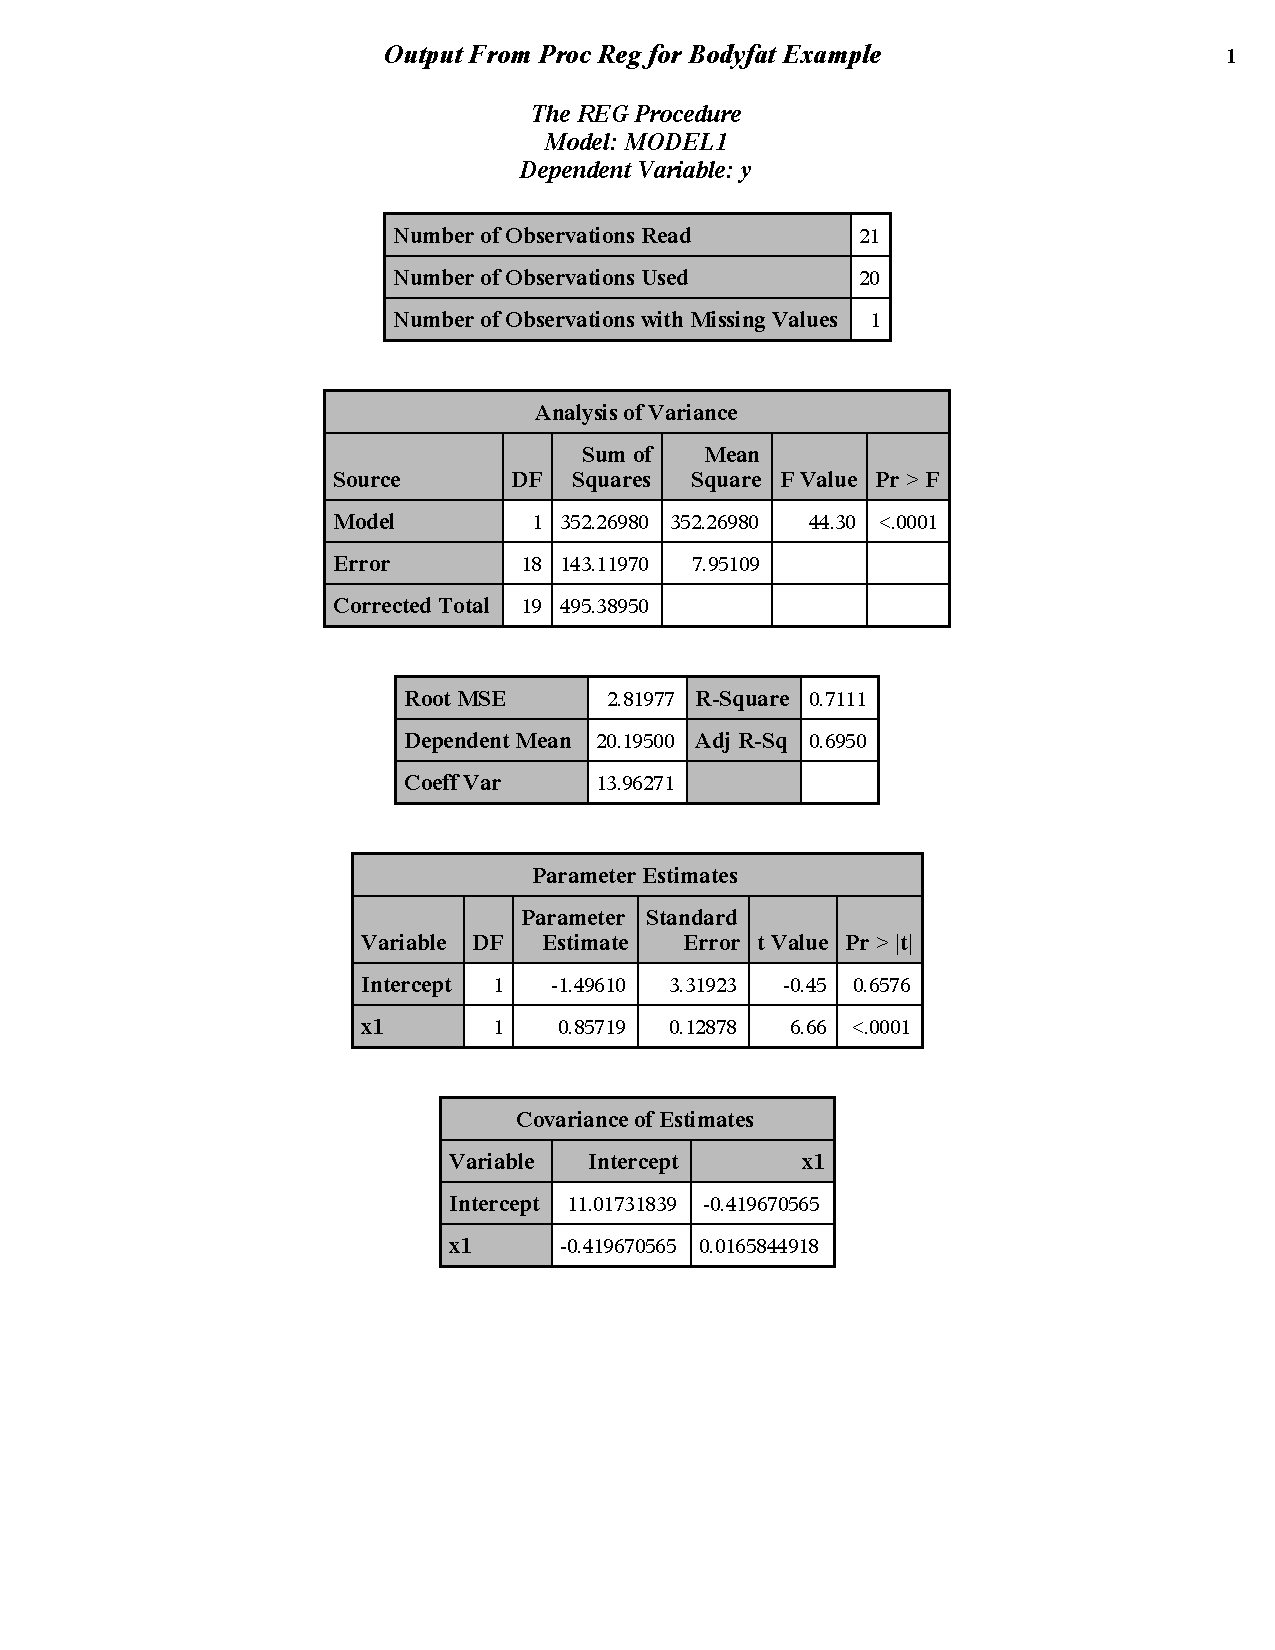
\includegraphics[page=1,scale=0.6,trim=40mm 30mm 20mm 10mm]{bodyfatexample}&\includegraphics[page=5,scale=0.6,trim=40mm 30mm 20mm 10mm]{bodyfatexample}\\
\end{tabular}
\end{center}

\textbf{To get the nested model $F$-ratio in SAS:}
\begin{small}
\begin{verbatim}
proc reg data=bodyfat;     model y=x1 x2 x3;
     test x2=0,x3=0;  run;
\end{verbatim}
\end{small}

\begin{center}
\includegraphics[page=4,scale=0.5,trim= 10mm 200mm 10mm 10mm]{bodyfatexampletriceps}
\end{center}

\newpage

\textbf{Test for midarm circumference:} - Let's also consider a test that midarm circumference is useful once triceps thickness and thigh circumference are in the model.

\begin{small}
\begin{verbatim}
proc reg data=bodyfat; model y=x1 x2/covb; run;
\end{verbatim}
\end{small}

\begin{flushleft}
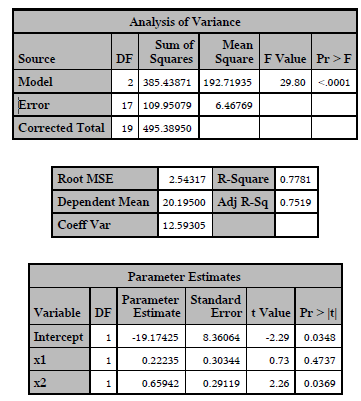
\includegraphics[scale=0.75]{bodyfatsnip}
\end{flushleft}


We can construct the F-test for nested models (lack of fit test):
\begin{eqnarray*}
\mbox{Model } A: \mu(x_1,x_2,x_3) & = & \beta_0 + \beta_1 x_1 + \beta_2 x_2 \\
\mbox{Model } B: \mu(x_1,x_2,x_3) & = & \beta_0 + \beta_1 x_1 + \beta_2 x_2 + \beta_3 x_3 
\end{eqnarray*} 
or the null hypothesis 
$$H_0: \beta_3=0 \ \ \mbox{  vs  } \ \ H_1: \beta_3\neq 0$$ 
(after accounting for $x_1$ and $x_2$.)
$$ F = \frac{(396.9-385.4)/1}{6.15} = \frac{11.5}{6.15}=1.87$$
At $\alpha=0.05$ the critical value is $F(0.05,~~~~~~~~ ,~~~~~~~~ ) = 4.49$.\\

Our conclusion about the hypotheses?\\~\\~\\~\\
%\textcolor{red}{\\That is, after accounting for the linear dependence between triceps/thigh circumference and bodyfat, there is no evidence for a linear association between mean bodyfat and midarm circumference.}

What do we notice about our $F$ statistic calculated and the test for $x_3$ in the parameter estimates table of the full model?$$t=-1.37~~~~~~~t^2=(-1.37)^2=1.8769$$
*****The tests in the parameter estimates table are really equivalent to doing the nested model selection tests removing only that predictor (called type III tests).


\newpage

\textbf{Full model questions}\\
Full model - Global p-value is significant\\~\\
None of the individual parameters have a significant p-value.\\~\\
Why?\\~\\~\\~\\~\\
%\textcolor{red}{\\Tests in parameter estimates tables are type III tests and so they are testing if each variable adds something once the others are all in the model.}

\textbf{Multicollinearity:} linear associations among the independent variables; causes problems such as inflated sampling variances for $\hat{\boldsymbol{\beta}}$.  (Which makes our t-stats smaller!)\\~\\

\begin{small}
\begin{verbatim}
ods graphics on;
proc corr plots=matrix;
var y x1 x2 x3;
run;
\end{verbatim}
\end{small}

\begin{center}
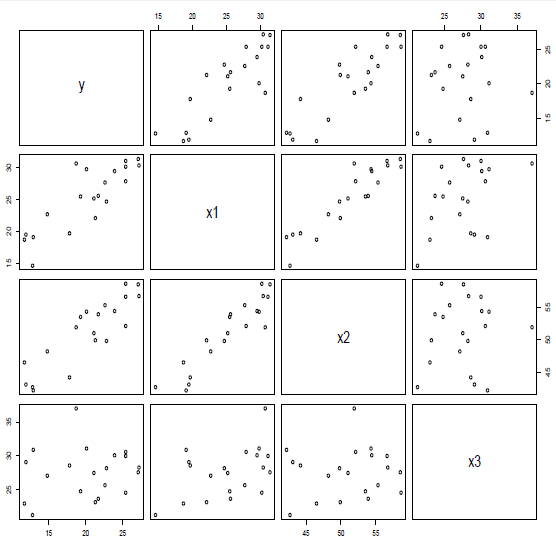
\includegraphics[height=4.7in,width=4.7in]{bodyfat}
\end{center}

\newpage

Consider all the `pairwise' correlations:

\normalsize
\begin{verbatim}
                Pearson Correlation Coefficients, N = 20 
                        Prob > |r| under H0: Rho=0
 
                       y            x1            x2            x3

        y        1.00000       0.84327       0.87809       0.14244
                                <.0001        <.0001        0.5491

        x1       0.84327       1.00000       0.92384       0.45778
                  <.0001                      <.0001        0.0424

        x2       0.87809       0.92384       1.00000       0.08467
                  <.0001        <.0001                      0.7227

        x3       0.14244       0.45778       0.08467       1.00000
                  0.5491        0.0424        0.7227              
\end{verbatim}
\large

Looking at the scatter plots and the correlation output:
\begin{itemize}
\item marginal (individual) associations between $y$ and $x_1$ and between $y$ and $x_2$ are highly significant
\item provides evidence of a strong ($r\approx 0.85$) linear association between average bodyfat and triceps skinfold
\item provides evidence of a strong ($r\approx 0.88$) linear association between average bodyfat and thigh circumference
\end{itemize}

Notice the scatter plot between $x_1$ and $x_2$ - there is a strong linear relationship.  \\~\\
This means that triceps skinfold thickness and thigh circumference are giving some of the same information.   That is, if you know triceps skinfold thickness is large then you know thigh circumference is large too... This can lead to issues when fitting a model.\\~\\

In the previous output we saw that a model with all three variables shows that once any two predictors are included, the third predictor does not add anything to the model.  This is most likely due to this multicollinearity.\\~\\

So what model to use? \\
General suggestion - Use the model that fits best, makes most sense scientifically, and also has the fewest number of predictors.\\~\\

\newpage

\Large\textbf{Automated Model Selection Techniques}\large\\

\textbf{Using proc reg to perform variable selection:}\\
We`ll discuss three hypothesis testing methods for selecting variables (there are many other ways to accomplish this we won`t discuss).\\

\textbf{Hypothesis Testing Methods:}
\begin{enumerate}
\item \textbf{Forward Selection} - Start with nothing and work forward.
	\begin{enumerate}
		\item Begin with a model with only $\beta_0$
		\item Fit SLR for all possible predictors and find p-values for each
		%Calculate $R(\beta_i|\beta_0)$ for all possible predictors and find p-values for each
		\item Take most significant p-value less than a cutoff (say 0.3), add predictor into model.  
		\item Say $\beta_j$ ($x_j$) was added in the last step, repeat above process with added predictor.  That is, calculate all MLR models with $x_j$ and one more predictor.
		\item Stop when no new predictors are below the cutoff or if the full model is selected.
	\end{enumerate}
\item \textbf{Backward Selection} - Start with everything and work backward. 
\begin{enumerate}
		\item Start with full model.
		\item Locate variable with largest p-value greater than a cutoff (say 0.1), remove that variable.
		\item Repeat until all p-values are less than the cut off or the null model (intercept only model) is chosen.
	\end{enumerate}
\end{enumerate}
\textbf{Fit Criterion Method}	
\begin{enumerate}\setcounter{enumi}{2}
\item \textbf{Subset Selection} - Compute all possible models, pick `best' according to a criterion.
\begin{enumerate}
		\item Fit all models under consideration.
		\item Compare each of the models using a criterion.  Choose `best' model.\\
Possible criteria include:
		\begin{itemize}
			\item $Adjusted~R^2 = 1-\frac{n-1}{n-p-1}(1-R^2)$ (takes into account the addition of more predictors)
			\item Mallow`s $C_P$, AIC, AICc, or BIC (all take into account the model complexity and model fit)
		\end{itemize}
	\end{enumerate}
\end{enumerate}
\textbf{Penalization Methods}
\begin{enumerate}\setcounter{enumi}{3}
\item More recent literature has focuses on penalization methods such as the LASSO, Elastic Net, SCAD, etc.  We will not discuss these in class.
\end{enumerate}

\newpage

\textbf{How to do these model selection methods in SAS?}
\begin{small}
\begin{verbatim}
proc reg data=bodyfat plots=none;  *run one of the model statements below;
    model y=x1 x2 x3/selection=cp ;                   
		model y=x1 x2 x3/selection=adjrsq; 
		model y=x1 x2 x3/selection=backward SLstay=0.1;  	   					
		model y=x1 x2 x3/selection=forward SLentry=0.3;   
run;
\end{verbatim}
\end{small}

\textbf{Subset Selection using Mallow's Cp}
\begin{flushleft}
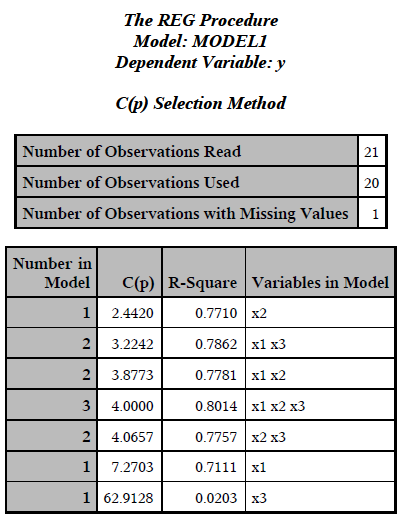
\includegraphics[scale=0.55]{bodyfatmallows}
\end{flushleft}

\textbf{Subset Selection using Adjusted $R^2$}
\begin{flushleft}
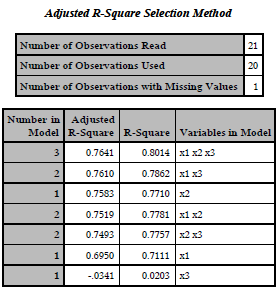
\includegraphics[scale=1]{bodyfatadjr2}
\end{flushleft}

\newpage

\textbf{Backward Selection}
\begin{flushleft}
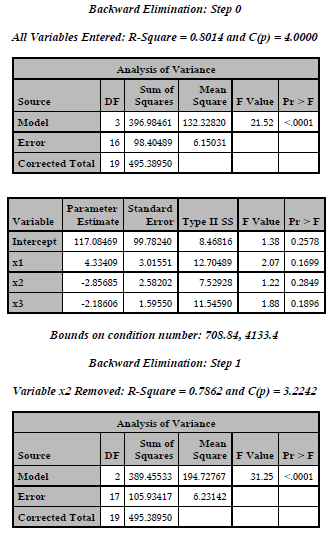
\includegraphics[scale=0.8]{bodyfatbackward1}\\
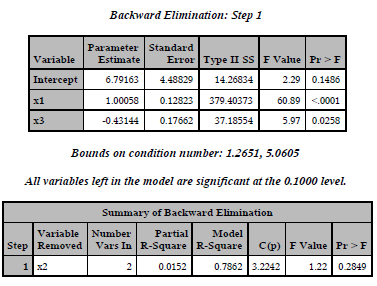
\includegraphics[scale=0.8]{bodyfatbackward2}
\end{flushleft}

\newpage

\textbf{Forward Selection}
\begin{flushleft}
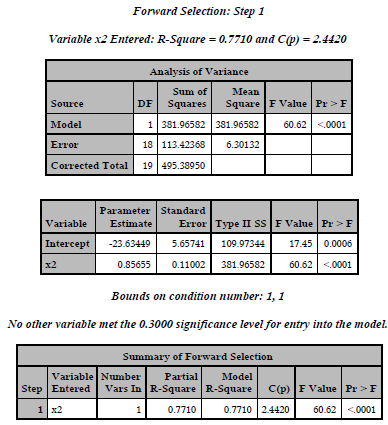
\includegraphics[scale=0.8]{bodyfatforward}
\end{flushleft}
~\\~\\~\\~\\
\textcolor{blue}{Note: the models selected by each procedure are not necessarily the same.  You should bring some subject matter knowledge into play here.}\\~\\

\newpage

\Large\textbf{Types of Sums of Squares}\large\\

\textcolor{blue}{If you notice, we now really have multiple tests for a given slope term.  A different test for each set of variables already being accounted for.  Let`s discuss this idea in more detail.}\\~\\

Given that we have 4 predictors, $x_1,x_2,x_3,x_4$, we really can have a number of tests based on nested models for each parameter.  \\

For instance, we can test 
$$H_0:\beta_4=0~~~~vs~~~~~H_A:\beta_4\neq 0$$ 
with
\begin{itemize}
\item No other variables in the model (SLR test)
\item After accounting for $x_1$ only
\item After accounting for $x_2$ only
\item After accounting for $x_1$ and $x_2$ 
\item After accounting for $x_1$ and $x_3$
\item After accounting for $x_1$, $x_2$, and $x_3$
\end{itemize}
Some of these tests can be easily found using different \textit{types of sums of squares}.\\

\begin{itemize}
\item Type I SS - \textbf{sequential} - test for adding the variable after all \textit{previous} variables are accounted for.\\
The order the variables are entered into the model determines the tests.\\
***** If you add up the type I SS for all parameters, you get the regression sum of squares (ignore the intercept type I SS if that is given).

\item Type II sums of squares - \textbf{partial} - test for adding the variable once all other terms not containing a function of that variable are accounted for (i.e. interactions/quadratics/etc). (We won't use these much.)

\item Type III sums of squares - \textbf{partial} - test for adding the variable after \textit{all} other terms in the model are accounted for.
\end{itemize}

The tests given for the parameter estimates are all type III tests.\\~\\
This is the test usually done to determine if a slope term has significance. \\~\\

However, Type I tests are very useful for model building. \\~\\

\newpage

For example, if we wanted to look at building a model for the bodyfat example and we thought the order of importance for the variables was $X_1$ (triceps), $X_3$ (midarm), and $X_2$ (thigh), we could get sequential tests for these models using type I sums of squares.\\

In SAS proc reg use the following code: (could be done in proc reg as well)\\
\begin{small}
\begin{verbatim}
proc glm data=bodyfat;
   model y=x1 x3 x2;   *order of variables important for type I SS!;
run;
\end{verbatim}
\end{small}

\begin{center}

\includegraphics[page=2,scale=0.7,trim= 10mm 60mm 10mm 10mm]{bodyfatexampletypeIglm}
\end{center}

These tests corresponding to the Type I SS use the \textit{full model} MS(E) rather than the MS(E) for the full model up to that point.  This test still works because MS(E) from each model is an unbiased estimate of $\sigma^2$.  The tests using the different MS(E) terms could give different results, but will usually agree.
\newpage

\Large\textbf{A linear regression example with a quadratic explanatory variable}\large\\
Data was collected on 5 kilometer run times.  The variables collected were age, sex, and pace.\\
\begin{small}
\begin{verbatim}
                  Obs    age    sex      race       pace

                    1     28     M     16.6833    5.38333
                    2     39     M     16.9500    5.46667
                    3     41     M     17.1333    5.51667
                    4     42     M     17.4000    5.61667
                  ...    ...   ...         ...        ...
                  157     52     F     46.8833    15.1000
                  158     10     F     53.6000    17.2667
                  159     10     F     53.6167    17.2667
                  160     81     M     54.3167    17.5000

\end{verbatim}
\end{small}
\begin{center}
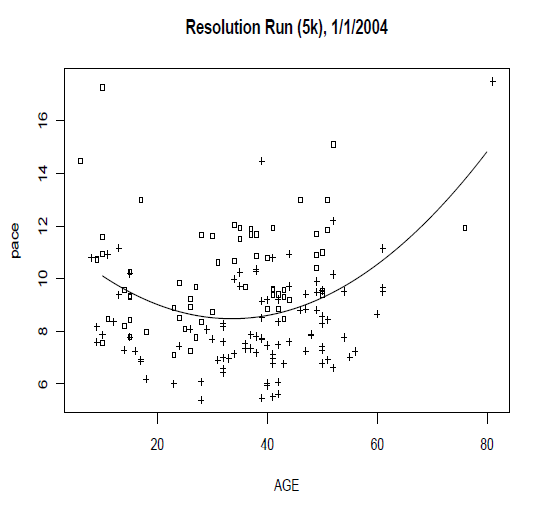
\includegraphics[scale=0.7]{res5k_quadratic}
\end{center}

Quadratic model for pace ($Y$) as a function of age ($x$):
$$ Y_i = \beta_0 + \beta_1 x_i + \beta_2 x_i^2 + E_i \ \ \mbox{ for }i=1,\ldots,160$$
where $E_i \iid N(0,\sigma^2)$.

\newpage

What does $\sigma^2$ represent in the model?\\~\\~\\~\\
%\textcolor{red}{\\The unknown error variance of paces given age $x$.}\\~\\
What do the parameters mean, i.e. what is their interpretation?\\~\\~\\~\\~\\~\\~\\~\\~\\
%\textcolor{red}{This is a quadratic equation and it is difficult to talk about the parameters separately.  You will usually want to discuss the entire curve at once.  However, we do know that the $\beta_2$ coefficient will shrink or expand the parabola as well as control concavity and the $\beta_1$ coefficient will move the parabola around.  Also, recall the minimum of the parabola will be at $-\frac{\beta_1}{2\beta_2}$. }\\~\\~\\~\\
 

We may want to do a LOF test with the SLR model 
$$ Y_i = \beta_0 + \beta_1 x_i + E_i \mbox{ for }i=1,\ldots,160$$

\begin{small}
\begin{verbatim}
proc glm data=running; 
   model pace=age age*age ; 
run;
\end{verbatim}
\end{small}

\begin{flushleft}
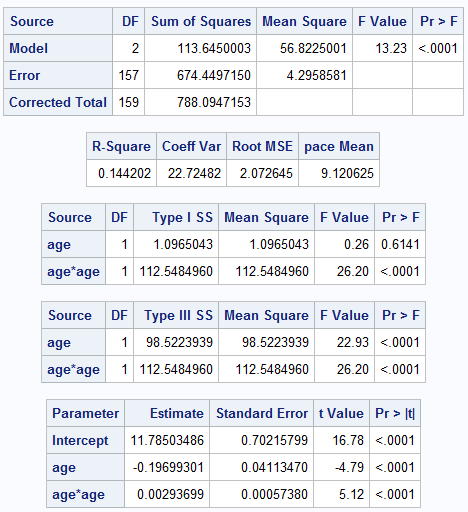
\includegraphics[scale=0.8]{resrunquadratic}
\end{flushleft}

\textcolor{blue}{Note with a little work we could get the exact SLR test given above (we`d have to solve for the MS(E) of that model for use in testing).}

Fitted models are:
\begin{eqnarray*}
\text{Model 1:} & & \hat\mu(age)=8.923 + 0.0056 age\\
\text{Model 2:} & & \hat\mu(age) = 11.785 - 0.197 age + 0.00294 age^2
\end{eqnarray*}

\begin{eqnarray*}
F & = & \frac{(SS(R)_{full}-SS(R)_{red})/1}{MS(E)_{full}} \\
  & = & \frac{(113.6-1.1)/1}{4.3} \\
  & = & \frac{(SS(E)_{red}-SS(E)_{full})/1}{MS(E)_{full}} \\
  & = & \frac{(787.0-674.4)/1}{4.3}\\
  & = & 26.2 \\
\end{eqnarray*}

Note: $\left(\frac{\hat\beta_{ 2}}{\hat{SE}}\right)^2 = (5.12)^2$\\

with $F(0.05,1,157)=3.90$.  Since $26.2 > > 3.9,$ we reject that the linear model is appropriate when compared to the quadratic model.  This is the same test as the t-test for age*age!

\begin{flushleft}
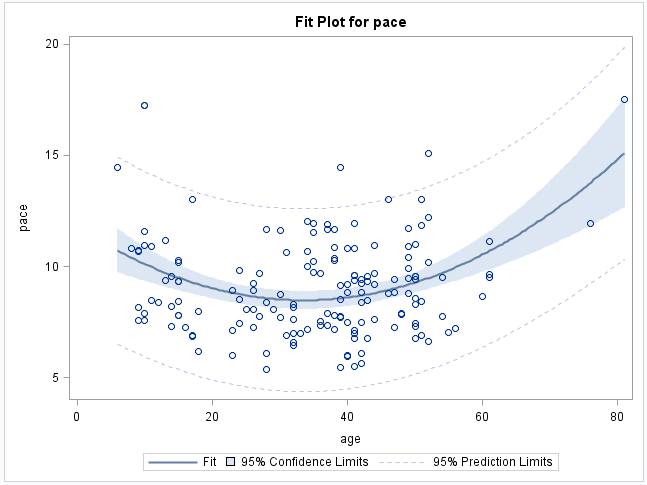
\includegraphics[scale=0.7]{resrunquadraticplot}
\end{flushleft}

\newpage


Note: The estimate of the minimum average pace is $-\hat{\beta}_1/(2\hat{\beta}_2)=-(-0.197)/(2*0.003)=32.83$.  \\~\\

We may want to make inference for the mean pace time of all individuals that are 32.83 years old.\\~\\

We can use the same ideas as before.  We really want to make inference for 
$$\hat{\mu}(32.83)=\hat{\beta}_0+\hat{\beta}_{1}32.83+\hat{\beta}_{2}32.83^2$$
which can be written in vector (linear combination) form as
$$\textbf{a}^{T}\boldsymbol{\hat{\beta}}$$ 
where 
$$\textbf{a}^{T}=(~~~~~~~~~~~~~~~~~~~~~~~~~~~~~~~~~~~~~~~~~~~~~~~~~~~~~~~~~~~~~)$$
%\textcolor{red}{$$\textbf{a}^{T}=(1~~~~32.83~~~~32.83^2)$$}

We can get the $\left(\textbf{X}^{T}\textbf{X}\right)^{-1}$ matrix by adding in `inverse' to the model statement
\begin{small}
\begin{verbatim}
 model pace=age age*age/inverse ; 
\end{verbatim}
\end{small}

\begin{center}
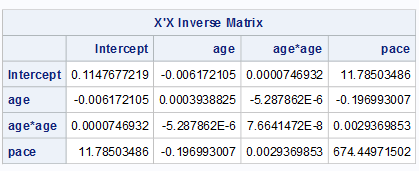
\includegraphics[scale=0.7]{xpxinverse}
\end{center}

A 95\% confidence interval for the mean pace time is given by
$$\textbf{a}^{T}\boldsymbol{\hat{\beta}}\pm t_{157,0.025}\sqrt{\textbf{a}^{T}\boldsymbol{\hat{\Sigma}}\textbf{a}}~~~~~~~~~~~~~~~~or~~~~~~~~~~~~~~\textbf{a}^{T}\boldsymbol{\hat{\beta}}\pm t_{157,0.025}\sqrt{MS(E)\textbf{a}^{T}\left(\textbf{X}^{T}\textbf{X}\right)^{-1}\textbf{a}}$$
\begin{flushleft}
$(1~~32.83~~32.83^2)\left(\begin{array}{c}11.785\\-0.197\\0.003\end{array}\right)\pm $
\end{flushleft}
\begin{flushright}
$1.975\sqrt{4.296(1~~32.83~~32.83^2)\left(\begin{array}{ccc} 0.115 &-0.006 &7.469E-5 \\-0.006& 3.94E-4 & -5.29E-6 \\ 7.47E-5 & -5.29E-6 &7.66E-8 \end{array}\right) \left(\begin{array}{c}1 \\32.83\\ 32.83^2\end{array}\right)}$
\end{flushright}

We are 95\% confident that the mean pace time for people that are 32.83 years old is between 8.077 and 8.890 minutes.\\

Note: Residual diagnostic shows slight non-normality.

\newpage

\Large\textbf{An Interaction Example}\large\\
A random sample of students taking the same exam yielded:
\begin{center}
\begin{tabular}{|c|c|c|} \hline
IQ & Study Time & Grade \\ \hline
105 & 10 & 75 \\
110 & 12 & 79 \\
120 & 6 & 68 \\
116 & 13 & 85 \\
122 & 16 & 91 \\
130 & 8 & 79 \\
114 & 20 & 98 \\
102 & 15 & 76 \\ \hline
\end{tabular}
\end{center}

We could consider an \textit{additive} model
$$Y_i=\beta_0+\beta_1x_{i1} +\beta_2x_{i2}+E_i$$~\\~\\~\\~\\
%\textcolor{red}{$$Grade=\beta_0+\beta_1IQ +\beta_2Time+Error$$~\\}
However, the grade on the exam might depend on how IQ and Study Time together. We may want to investigate this \textbf{interaction} effect - IQ*Time.\\~\\

Recall: Interaction implies that the way one variable effects the response depends on the level of the other variable.\\

Here, what does that mean?\\~\\~\\~\\~\\~\\~\\
%\textcolor{red}{\\~\\The effect IQ has on your Grade differs depending on your Study Time.  Or equivalently, the effect Study Time has on Grade differs depending on your IQ.}\\~\\

Consider the \textit{interaction} model
$$Y_i=\beta_0+\beta_1X_{i1} +\beta_2X_{i2}+\beta_3X_{i1}X_{i2}+E_i$$~\\~\\~\\~\\
%\textcolor{red}{$$Grade=\beta_0+\beta_1IQ +\beta_2Time+\beta_3Time*IQ+Error$$}

\newpage

The following models were fit in SAS:
\begin{small}
\begin{verbatim}
proc glm data=test;                        proc glm data=test;
model Grade=IQ|Time;                       model Grade=Time|IQ;
run;                                       run;
\end{verbatim}
\end{small}

\begin{flushleft}
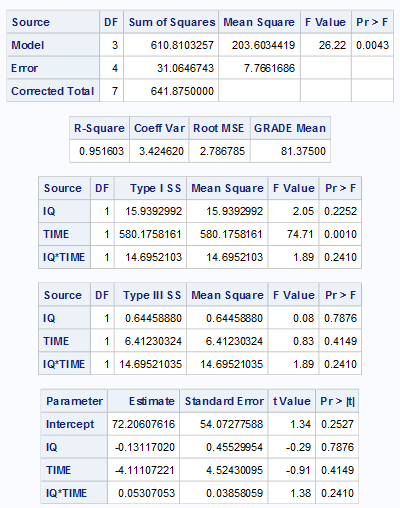
\includegraphics[scale=0.9]{Testoutput}\\
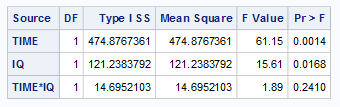
\includegraphics[scale=0.9]{Testoutput2}
\end{flushleft}

\newpage

Notice that our explanatory variables do not have an independent effect on the response.
$$ \widehat{Mean Grade} = 72.21 - 0.13*IQ - 4.11*Time + 0.0531*IQ*Time$$ 
Now if IQ = 100 we get
$$ \widehat{Mean Grade} = (72.21 - 13.1) + (- 4.11 + 5.31)*Time= 59.11+1.20*Time $$
and if IQ = 120 we get
$$ \widehat{Mean Grade} = (72.21 - 15.7) + (- 4.11 + 6.37)*Time =56.51+2.26*Time$$
Thus we expect an extra hour of study to increase the grade by 1.20 points for someone with IQ = 100 and by 2.26 points for someone with IQ = 120 if we use this interaction model.\\~\\

%\textcolor{red}{Think about how this type of effect could come into play in your research.}

Generally, we can interpret the (true) $\beta$ parameters in the model as:
\begin{itemize}
\item $\beta_0$ - Average value of Grade when IQ and Study Time are 0
\item $\beta_1$ - Average change in Grade for a unit increase in IQ when Study Time is 0
\item $\beta_2$ - Average change in Grade for a unit increase in Study Time when IQ is 0
\item $\beta_3x_2$ - Average change in the slope for IQ (or Study Time) for a given value of Study Time (or IQ).
\end{itemize}
The interpretation of the interaction `slope' can be seen by looking at the following:
$$\mu(x_1+1,x_2)-\mu(x_1,x_2)=\beta_0+\beta_1(x_1+1)+\beta_2x_2+\beta_3(x_1+1)(x_2)-\beta_0-\beta_1x_1-\beta_2x_2-\beta_3x_1(x_2)$$
$$=\beta_1+\beta_3x_2$$
So $\beta_3x_2$ is the amount the slope for $x_1$ changes per unit change in $x_1$ for a fixed constant value of $x_2$.\\~\\

Note:  You may want to center your predictors to make the parameter interpretations more meaningful.\\~\\

The global p-value is significant, but none of our individual terms are.   We can use the type I Sums of Squares to do model building!!  What model would you choose and why?


\newpage

\Large\textbf{Polynomial Contrasts (Optional Reading)}\large\\
Often in One-Way ANOVA with a single factor, the factor is not categorical - rather it is numeric but observed at only a few levels.\\~\\

If this is the case we can test for polynomial relationships as opposed to the One-Way ANOVA model.\\~\\

With $t$ levels, we can fit any polynomial of degree $t-1$ or less.  (Polynomial of degree $t-1$ is equivalent to fitting the One-Way ANOVA model.) \\~\\

That is, every polynomial model of degree $t-2$ or less is nested in the full ANOVA model!\\~\\

Example: A poultry science experiment measures bodyweights of chickens from $t=4$ diet groups.  Diets are characterized by protein concentration in diet.
\begin{itemize}
\item Response $Y$ = 21-day bodyweights of chickens 
\item A balanced CRD was done with diet and $N=72$ total chickens.  (Implying $n=18$).
\end{itemize}
Experiment Summary:
\begin{center}
\begin{tabular}{ccc}
diet group & $x$: level of protein & diet mean $\bar{y}_{i+} $\\\hline
1 &              21.8         & 994.9       \\
2 &              23.5         & 1000.6 \\
3 &              25.2         & 1025.8 \\
4 &              26.9         & 1056.0\\ 
\hline
\end{tabular}
\end{center}
Here we can see that our factor is actually numeric but measured at only 4 levels. 

\newpage

Consider the One-way ANOVA model using diet and the Linear Regression model cubic in protein:
\begin{small}
\begin{verbatim}
proc glm data=chickens; class diet;
model gain=diet; run;

proc glm data=chickens;
model gain=protein protein*protein protein*protein*protein; run;
\end{verbatim}
\end{small}

\begin{flushleft}
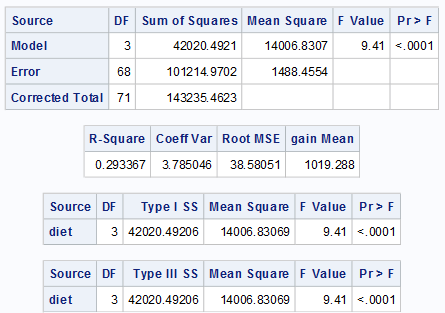
\includegraphics[scale=1]{ChickensGLM}\\
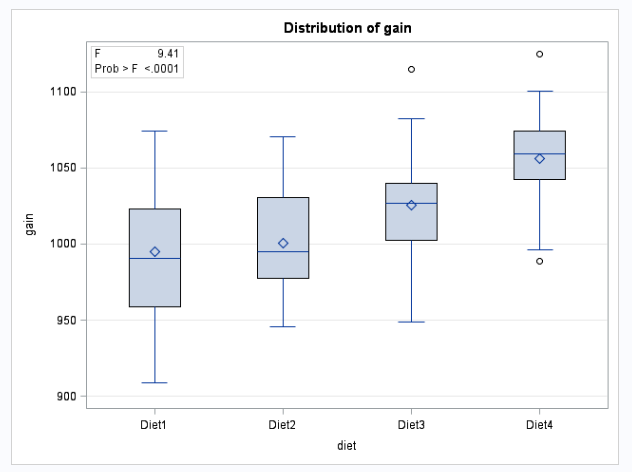
\includegraphics[scale=0.5]{ChickensBoxPlot}
\end{flushleft}

\newpage

\begin{flushleft}
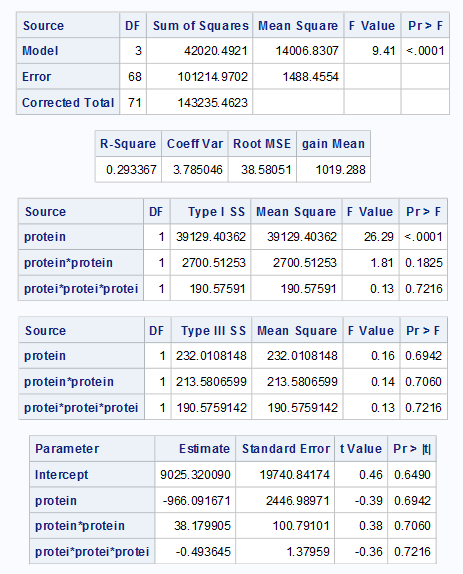
\includegraphics[scale=0.8]{ChickensGLM2}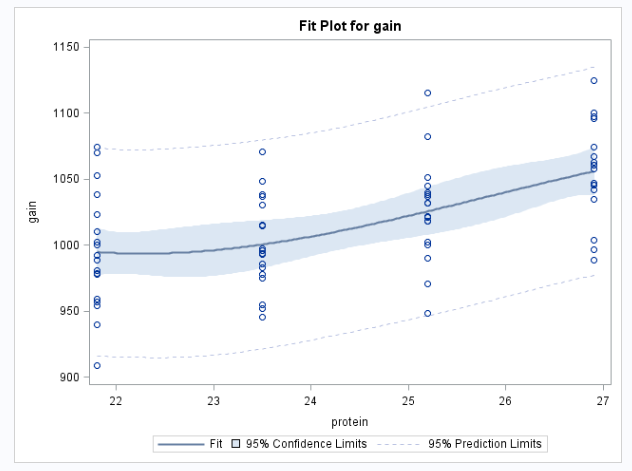
\includegraphics[scale=0.5]{ChickensScatter}
\end{flushleft}

Investigate the two ANOVA tables.  Also inspect the Type I Sums of Squares for the MLR model, these would be useful in model building! \\~\\
We can test for the adequacy of a model linear or quadratic in protein rather than the full ANOVA (equivalent to the cubic model).\\~\\

\newpage 
If we have equally spaced levels (differences between levels all the same), we can actually write down the different polynomial parts in terms of contrasts.  Below gives the contrasts you would use for equally spaced levels for 3, 4, or 5 levels.
\begin{center}
\begin{tabular}{ccc|ccccc|c}
Factor& Poly.& & \multicolumn{5}{c|}{Coefficients for} & \\
levels & Degree & contrast & $\bar{y}_{1+}$ & $\bar{y}_{2+}$ & $\bar{y}_{3+}$ & $\bar{y}_{4+}$ & $\bar{y}_{5+}$ & $SS(\hat\theta_i)$\\ \hline
3 & 1 &$\hat\theta_1$& -1 & 0 & 1 & & & $R(\beta_1|\beta_0)$\\
  & 2 &$\hat\theta_2$& 1 & -2 & 1 & & & $R(\beta_2|\beta_0,\beta_1)$\\ \hline
4 & 1 &$\hat\theta_1$& -3 & -1 & 1 & 3 & & $R(\beta_1|\beta_0)$\\
  & 2 &$\hat\theta_2$& 1 & -1 & -1 & 1 & & $R(\beta_2|\beta_0,\beta_1)$\\ 
  & 3 &$\hat\theta_3$& -1 & 3 & -3 & 1 & & $R(\beta_3|\beta_0,\beta_1,\beta_2)$\\  \hline
5 & 1 &$\hat\theta_1$& -2 & -1 & 0 & 1 & 2 & $R(\beta_1|\beta_0)$\\
  & 2 &$\hat\theta_2$& 2 & -1 & -2 & -1 & 2 & $R(\beta_2|\beta_0,\beta_1)$\\
  & 3 &$\hat\theta_3$& -1 & 2 & 0 & -2 & 1 & $R(\beta_3|\beta_0,\beta_1,\beta_2)$\\
  & 4 &$\hat\theta_4$& 1 & -4 & 6 & -4 & 1 & $R(\beta_4|\beta_0,\beta_1,\beta_2,\beta_3)$\\ \hline
\end{tabular}
\end{center}

Rightmost column indicates extra SS in MLR of the form
$$\mu(x) = \beta_0 + \beta_1 x + \beta_2 x^2 + \cdots.$$
The contrast corresponding to a polynomial of degree $p$
can be used to test for a $p^{th}$ degree association:

\begin{itemize}
\item large $|\hat\theta_1|$ indicates
linear association between $y$ and $x$.
\item large $|\hat\theta_2|$ indicates
quadratic association between $y$ and $x$.
\item large $|\hat\theta_3|$ indicates 
cubic association between $y$ and $x$.
\end{itemize}

\begin{small}
\begin{verbatim}
proc glm data=chickens; class diet; model gain=diet;
contrast 'linear' diet -3 -1 1 3;
contrast 'quadratic' diet 1 -1 -1 1;
contrast 'cubic' diet -1 3 -3 1; run;
\end{verbatim}
\end{small}

\begin{center}
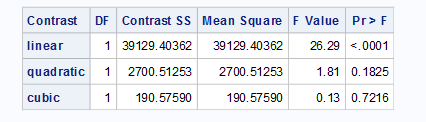
\includegraphics[scale=0.8]{ChickensGLM3}
\end{center}

Note the equivalence between this output and the linear regression model cubic in protein.  Conclusion? \\~\\
 Go ahead and use the linear model rather than the full ANOVA.  No need to look at pairwise comparisons etc.\\~\\

\textbf{$F$-ratio for lack-of-fit:}\\ 
To test for lack-of-fit of a polynomial ({\em reduced}) model of degree $p$, use extra sum-of-squares F-ratio on $t-1-p$ and $N-t$ $df$:
$$ F=\frac{SS(\mbox{lack of fit})/(t-1-p)}{MS(E)_{full}}$$
where
\begin{eqnarray*}
SS(\mbox{lack-of-fit})  &=&  SS(Trt)-SS(R)_{poly} \\
&=&  SS(E)_{poly}-SS(E)_{full}
\end{eqnarray*}

For illustration purposes (i.e. this isn't necessary), let's test if the quadratic model is sufficient or if the full ANOVA model is necessary.\\

$$SS(\mbox{lack-of-fit})=42020.49-(39129.40+2700.51)=190.58$$
$$MS(E)_{full}=1488.46$$
This implies
$$F=\frac{SS(\mbox{lack of fit})/(4-1-2)}{MS(E)_{full}}=190.58/1488.46=0.128$$
Fail to reject that the full ANOVA model is necessary.  That is, the quadratic model does not suffer from lack of fit.
